\documentclass[acmsmall,screen,review]{acmart}

\AtBeginDocument{%
  \providecommand\BibTeX{{%
    Bib\TeX}}}


\setcopyright{acmcopyright}
\copyrightyear{2018}
\acmYear{2018}
\acmDOI{XXXXXXX.XXXXXXX}


%%
%% These commands are for a JOURNAL article.
\acmJournal{JACM}
\acmVolume{37}
\acmNumber{4}
\acmArticle{111}
\acmMonth{8}


%\usepackage{cite}
\usepackage{amsmath,amsfonts}
\usepackage{algorithmic}
\usepackage{graphicx}
\usepackage{textcomp}
\usepackage{xcolor}
\usepackage{xspace}
\usepackage{fontawesome}
\usepackage{multirow}
\usepackage{rotating}
\usepackage{tikz}
\usepackage{soul}
\usepackage{makecell}
\usepackage{url}
\usepackage{enumitem}
\usepackage{booktabs}
\usepackage{fontawesome}
\usepackage{graphicx}
\usepackage{hyperref}
\usepackage{pifont}
\usepackage{multicol}
\usepackage{tcolorbox}
\usepackage{pifont}% http://ctan.org/pkg/pifont
\newcommand{\cmark}{\ding{51}}%
\newcommand{\xmark}{\ding{55}}%


\newcommand\TODO[1]{\textcolor{red}{#1}}
\newcommand\REMOVE[1]{\textcolor{red}{\st{#1}}}
\newcommand\ANTONIO[1]{\textcolor{blue}{{ANTONIO}{#1}}}
\newcommand\LUCA[1]{\textcolor{green}{{LUCA}{#1}}}
\newcommand\GABRIELE[1]{\textcolor{red}{{GABRIELE}{#1}}}
\newcommand{\ie}{\emph{i.e.,}\xspace}
\newcommand{\eg}{\emph{e.g.,}\xspace}
\newcommand{\etc}{etc.\xspace}
\newcommand{\etal}{\emph{et~al.}\xspace}
\newcommand{\secref}[1]{Section~\ref{#1}\xspace}
\newcommand{\chapref}[1]{Chapter~\ref{#1}\xspace}
\newcommand{\appref}[1]{Appendix~\ref{#1}\xspace}
\newcommand{\figref}[1]{Fig.~\ref{#1}\xspace}
\newcommand{\listref}[1]{Listing~\ref{#1}\xspace}
\newcommand{\tabref}[1]{Table~\ref{#1}\xspace}
\newcommand{\tool}[1]{{\sc #1}\xspace}
\newcommand{\highlight}[1]{{\color{purple} \textbf{#1}}}
\newcommand{\approach}{LEONID\xspace} %Log gEneratiON using Information retrieval and Deep learning
\newcommand{\java}{\emph{Java}\xspace}


\newcommand*\circled[1]{\tikz[baseline=(char.base)]{
		\node[shape=circle,fill,inner sep=0.8pt] (char) {\textcolor{white}{#1}};}}

\def\BibTeX{{\rm B\kern-.05em{\sc i\kern-.025em b}\kern-.08em
		T\kern-.1667em\lower.7ex\hbox{E}\kern-.125emX}}

\definecolor{gray50}{gray}{.5}
\definecolor{gray40}{gray}{.6}
\definecolor{gray30}{gray}{.7}
\definecolor{gray20}{gray}{.8}
\definecolor{gray10}{gray}{.9}
\definecolor{gray05}{gray}{.95}

\newlength\Linewidth
\def\findlength{\setlength\Linewidth\linewidth
	\addtolength\Linewidth{-4\fboxrule}
	\addtolength\Linewidth{-3\fboxsep}
}
\newenvironment{rqbox}{\par\begingroup
	\setlength{\fboxsep}{5pt}\findlength
	\setbox0=\vbox\bgroup\noindent
	\hsize=0.95\linewidth
	\begin{minipage}{0.95\linewidth}\normalsize}
	{\end{minipage}\egroup
	\textcolor{gray20}{\fboxsep1.5pt\fbox{\fboxsep5pt\colorbox{gray05}{\normalcolor\box0}}}
	\endgroup\par\noindent
	\normalcolor\ignorespacesafterend}

\definecolor{lightergray}{rgb}{0.9,0.9,0.9}
\newtcolorbox{resultbox}{colback=lightergray, arc=0.5mm, top=2mm, bottom=2mm, left=2mm, right=2mm}

\begin{document}


\title{Log Statements Generation via Deep Learning: Widening the Support Provided to Developers}


\author{Antonio Mastropaolo}
\affiliation{%
  \institution{SEART @  Software Institute, Universit\`a della Svizzera italiana}
  \city{Lugano}
  \country{Switzerland}
}
\email{antonio.mastropaolo@usi.ch}

\author{Valentina Ferrari}
\affiliation{%
 \institution{SEART @  Software Institute, Universit\`a della Svizzera italiana}
  \city{Lugano}
\country{Switzerland}
}
\email{valentina.ferrari@usi.ch}

\author{Luca Pascarella}
\affiliation{%
  \institution{}
   \city{Zurich}
 \country{Switzerland}
}
  \email{.......}
\author{Gabriele Bavota}
\affiliation{%
  \institution{SEART @  Software Institute, Universit\`a della Svizzera italiana}
   \city{Lugano}
 \country{Switzerland}
} 
\email{gabriele.bavota@usi.ch}



\renewcommand{\shortauthors}{Mastropaolo et al.}



\begin{abstract}
	Logging helps keeping track of events occurring during software execution. Previous work stressed the challenges developers face when logging. These include: \emph{where} to log, \emph{what} information to log, and which \emph{log level} to use (\eg info, fatal). To support developers in all these decisions, we presented LANCE, a deep learning (DL)-based approach to automatically inject a log statement in a given Java method. While being the state-of-the-art in the automation of logging activities, LANCE suffers of two major limitations. First, given a method as input, LANCE always assumes that it requires the injection of exactly \emph{one} new log statement, even in cases in which \emph{no} additional log statements would be needed or \emph{multiple} log statement would be required. Second, LANCE is only able to generate meaningful log messages in 15.2\% of cases. In this work, we study how to address these limitations to widen the support provided to developers in terms of logging automation. We start by replicating LANCE on a dataset 3.6 times larger than the one used in our previous study.
	Then, we present \approach, an extension of LANCE which is able to (i) decide whether a given Java method would actually benefit from the injection of log statements (or if, instead, those are not needed); and (ii) support the injection of multiple log statements if needed, deciding how many statements are needed, where they should be placed, and what they should log. Finally, we also tried to boost the generation of meaningful log messages by combining information retrieval (IR) and DL. Our results show that: (i) \approach can accurately discriminate between methods needing and not needing the addition of log statements; (ii) \approach can support, when needed, the injection of multiple log statements in a given method with, however, a loss in performance as compared to the simpler single-log injection problem addressed by LANCE; (iii) by just increasing the size of the training dataset, LANCE's ability to predict meaningful log messages improves by a factor of two, approaching 30\%; (iv) \approach can only slightly improve the performance of LANCE in generating meaningful log messages thanks to the combination of DL and IR, thus calling for additional research on this specific problem.
\end{abstract}


\begin{CCSXML}
  <ccs2012>
  <concept>
  <concept_id>10011007.10011006.10011073</concept_id>
  <concept_desc>Software and its engineering~Software maintenance tools</concept_desc>
  <concept_significance>500</concept_significance>
  </concept>
  </ccs2012>
\end{CCSXML}

\ccsdesc[500]{Software and its engineering~Software maintenance tools}

\ccsdesc[500]{Software and its engineering}
\ccsdesc[300]{Software development techniques}


\keywords{software logging, pre-trained models of code}

%\received{20 February 2007}
%\received[revised]{12 March 2009}
%\received[accepted]{5 June 2009}
\maketitle

% !TEX root = main.tex
%%%%%%%%%%%%%%%%%%%%%%%%%%%%%%%%%%%%%%%%
%%%%%%%%%%%%%%%%%%%%%%%%%%%%%%%%%%%%%%%%
\section{Introduction} \label{sec:intro}
%%%%%%%%%%%%%%%%%%%%%%%%%%%%%%%%%%%%%%%%
%%%%%%%%%%%%%%%%%%%%%%%%%%%%%%%%%%%%%%%%

% !TEX root = ../main.tex

% Zhu \etal~\cite{zhu2015learning} \textsc{LogAdvisor}
% Yao \etal~\cite{yao2018log4perf} \textsc{Log4Perf}


\begin{table*}[]
\centering
    \caption{Number of methods in the datasets used in our study}
        \label{tab:ds-summary-1}
\begin{tabular}{lll|ccc|cc|c}

\toprule
\multirow{2}{*}{\textbf{Ref.}}                  & \multirow{2}{*}{\textbf{Venue}} & \multirow{2}{*}{\textbf{Name}} & \multicolumn{3}{c|}{\textbf{Log}} & \multicolumn{2}{c|}{\textbf{Log injection}} & \multirow{2}{*}{\textbf{Need for log statements}} \\
                                                &                                 &                                & Level    & Position   & Message   & Single              & Multiple              &                                                  \\\midrule
Zhu \etal~\cite{zhu2015learning}                & ICSE 2015                       & \textsc{LogAdvisor}            & \xmark   & \cmark     & \xmark    & \cmark              & \xmark                &  \xmark                                          \\
Yao \etal~\cite{yao2018log4perf}                & ICPE 2018                       & \textsc{Log4Perf}              & \xmark   & \cmark     & \xmark    & \cmark              & \xmark                &  \cmark                                          \\
Mizouchi \etal~\cite{mizouchi2019padla}         & ICPC 2019                       & \textsc{PADLA}                 & \cmark   & \xmark     & \xmark    & \cmark              & \cmark                &  \xmark                                          \\
Li \etal~\cite{li2020shall}                     & ASE 2020                        & \textsc{}                      & \xmark   & \cmark     & \xmark    & \cmark              & \xmark                &  \xmark                                          \\
Li \etal \cite{li2021deeplv}                    & ICSE 2021                       & \textsc{DeepLV}                & \cmark   & \cmark     & \xmark    & \cmark              & \xmark                &  \xmark                                          \\
Mastropaolo \etal~\cite{mastropaolo2022using}   & ICSE 2022                       & \textsc{LANCE}                 & \cmark   & \cmark     & \cmark    & \cmark              & \xmark                &  \xmark                                          \\
Our tool \cite{replication_package}             & Under review                    & \textsc{LEONID}                & \cmark   & \cmark     & \cmark    & \cmark              & \cmark                &  \cmark                                          \\
\bottomrule
\end{tabular}
\end{table*}

The practice of injecting log statements in applications' code is widely adopted both in industry and open source projects \cite{oliner2012advances}. Indeed, log statements are instrumental to support several software-related activities, including program comprehension and debugging \cite{lu2017log,gurumdimma2016crude}. Given its popularity, it comes without surprise the proliferation of libraries to support logging activities: just for \java, some possible options are Log4j \cite{log4j}, JCL \cite{jcl}, slf4j \cite{slf4j}, and logback \cite{logback}.

While logging is usually perceived as a good practice, it comes with its own drawbacks: Excessive logging could negatively impact performance and, if not carefully conceived, log statements can result in security issues such as providing access to user credentials or sensitive information. 

Also, researchers documented several bad practices that should be avoided while logging code \cite{Chen:icse2017,Li:icse2019}. 
In general, logging poses several challenges to software developers. First, they need to decide \emph{what to log}, by finding the right amount of log statements needed in the application without, however, flooding it with useless log statements. Second, developers must \emph{log at the proper level}, namely, select the proper log level for each entry (\eg info, warning, error). Third, log statements must be accompanied by \emph{meaningful and informative} log messages that can be easily understood.

To support developers in these activities, researchers proposed techniques and tools automating specific aspects of logging, such as recommending (i) where/what to log \cite{yuan2010sherlog,jia2018smartlog,li2018studying,harty2021logging,li2020shall}, and (ii) the right level to use for a given log statement \cite{yuan2012characterizing,oliner2012advances,li2017log,li2020qualitative,li2021deeplv}. Recently, Mastropaolo \etal \cite{mastropaolo2022using} presented LANCE, an approach built on top of a Text-To-Text-Transfer-Transformer (T5) deep learning (DL) model \cite{raffel2019exploring} trained to generate and inject a complete log statement in a \java method provided as input. The T5 model has been pre-trained on a set of $\sim$6.8M \java methods using the classic ``masked language modeling'' objective \cite{raffel2019exploring}. In the case of LANCE, this means that during pre-training the model is provided as input a \java method with 15\% of its tokens masked and it is expected to predict the masked ones. Such a pre-training task provides T5 with knowledge about the language of interest (\ie \java). Once pre-trained, the model has been fine-tuned for the specific task of interest. In this case, the authors selected $\sim$62k \java methods and removed from them exactly one log statement asking the model to generate and inject it, thus deciding \emph{where} to log (\ie in which part of the method), which \emph{log level} to use, and \emph{what} to log (\ie generate a meaningful log message in natural language). LANCE is the first approach that supports developers in all these activities. The presented empirical evaluation showed that LANCE was able to correctly predict the appropriate location of a log statement and its level in $\sim$66\% of cases, while the approach struggled in predicting a meaningful log message, being successful in 15.2\% of test instances. While LANCE represents a substantial step ahead in logging automation, it comes with some limitations. First, it assumes that only one log statement is needed in a \java method provided as input. This is due to the training procedure employed by the authors that asks the model to always generate a single log statement. While such an assumption simplifies the addressed problem, it is not empirically supported, since $\sim$86\% of \java methods in our dataset makes use of more than one log statement. Second, given a \java method, LANCE cannot even assess whether log statements are needed at all. 

\eject

Indeed, in some cases, enough log statements may be already present in the method or, maybe, the method does not feature statements that would benefit from logging. Finally,  while LANCE achieves good performance in predicting the log statement location and level, it showed substantial limitations in synthesizing meaningful natural language log messages. In this work we study how to partially address these limitations.

We start replicating LANCE by training and testing it on a dataset 3.6 times larger than the one used by Mastropaolo \etal \cite{mastropaolo2022using} (230k training instances \emph{vs} 63k). Besides being larger, our dataset, as we will explain, features a more variegate set of log statements. Then, we present \approach as an extension of LANCE able to (i) discriminate between methods \emph{needing} and \emph{not needing} the injection of new log statements; and (ii) in case a need for log statements is identified, \approach, differently from LANCE, can decide the proper number of log statements to inject (which can be higher than one) and properly place them in the correct position. We found that \approach can correctly predict the need for log statements with an accuracy higher than 90\%. Also, when log statements are needed, it can generate and inject in the right position multiple complete log statements in $\sim$17\% of cases, against the $\sim$27\% success rate achieved in the simpler scenario of single-log injection (\ie the same problem addressed by LANCE).   

Finally, in \approach, we attempted to improve the performance achieved in the generation of meaningful log messages by exploiting a combination of DL and Information Retrieval (IR). Indeed, based on the results reported in \cite{mastropaolo2022using}, the generation of log messages really looked like the Achilles' heel of DL-based log generation. However, we found that by simply increasing the size of the training dataset, the ability of LANCE in predicting meaningful log messages is boosted to 30\% (+100\% as compared to what reported in \cite{mastropaolo2022using}). Starting from this level of performance, the combination of DL and IR we propose in \approach only provides a further +5\% relative improvement (31.55\%) in log message generation, pointing to the need for additional research on this problem.

\tabref{tab:sota} shows how \approach widens the support provided to developers in the automation of logging activities. Indeed, it is the only one deciding whether log statements are needed in a method and, in case of positive answer, synthesizing multiple and complete log statements, and injecting them in the correct position. 

%Increasing the complexity of the problem is likely to result in a decrease of accuracy. However, \approach exploits a new fine-tuning strategy combining DL and Information Retrieval (IR) to boost the prediction accuracy when it comes to the most challenging sub-problem involved in log injection: the generation of a meaningful log message. To explain our fine-tuning training procedure let us indicate with $<$$m_i$, $LS=\{ls_1, ls_2, \dots, ls_n\}$$>$ a training instance in our dataset, with $m_i$ being a Java method from which we removed $n$ log statements and $LS$ being the set of removed statements the model is expected to generate. We identify in the training set the top-$k$ methods being most similar to $m_i$ and extract the set of log messages $M$ used in them. We use $M$ to augment our training instance, that becomes a triplet composed by $<$$m_i$, $LS=\{ls_1, ls_2, \dots, ls_n\}$, $M$$>$. The idea is that T5 can learn how to write a meaningful log message for $LS$ by looking at examples of log messages ($M$) used in methods similar to the one it is provided as input ($m_i$). While testing our approach on a previously unseen method $m_j$, we follow the same procedure by identifying the top-$k$ most similar methods in our training set.
% !TEX root = main.tex
%%%%%%%%%%%%%%%%%%%%%%%%%%%%%%%%%%%%%%%%
%%%%%%%%%%%%%%%%%%%%%%%%%%%%%%%%%%%%%%%%
\section{\approach} \label{sec:t5}
%%%%%%%%%%%%%%%%%%%%%%%%%%%%%%%%%%%%%%%%
%%%%%%%%%%%%%%%%%%%%%%%%%%%%%%%%%%%%%%%%

We start by providing an introduction to the T5 model we use (\secref{sub:t5}). Then, we describe how we built the datasets used for the different training phases we dealt with (\secref{sub:datasets}).  \secref{sec:training} will then explain how we used these datasets to run the actual training process.


\subsection{Text-to-Text-Transfer-Transformer (T5)}
\label{sub:t5}
T5 has been introduced by Raffel \etal \cite{raffel2019exploring} as a Transformer \cite{vaswani2017attention} model to support multitask learning in the domain of NLP (Natural Language Processing). The idea behind the T5 model is to reframe NLP tasks in a unified text-to-text format in which the input and output of the model are text strings. This implies that a single model can be trained to translate across languages (\eg from English to Spanish) and to autocomplete sentences. The training of T5 includes two phases. The first is the \textit{pre-training}, in which the model is trained with a self-supervised objective to acquire general knowledge about the language(s) of interest. In our example, this may mean providing as input to the model English sentences having a subset of their words masked and asking the model to generate as output the masked words. Being self-supervised (\ie the training instances can be automatically generated by masking random words) the pre-training can usually be performed on large-scale datasets. Once pre-trained, T5 can be fine-tuned to support specific tasks with supervised training objectives. This means, for example, providing it with pairs of sentences $<$\emph{english}, \emph{spanish}$>$.

In our work, we rely on the same T5 architecture (\ie T5$_{small}$) that has been exploit by Mastropaolo \etal \cite{mastropaolo2022using} in LANCE. T5\textsubscript{\textit{small}} is characterized by six blocks for encoders and decoders. The feed-forward networks in each block consist of a dense layer with an output dimensionality ($d_{ff}$) of 2,048. The \textit{key} and \textit{value} matrices of all attention mechanisms have an inner dimensionality ($d_{kv}$) of 64, and all attention mechanisms have eight heads. All the other sub-layers and embeddings have a dimensionality ($d_{model}$) of 512. The code implementing T5 is available in our replication package \cite{replication}.


\subsection{Datasets Needed for Training, Validation, and Testing}
\label{sub:datasets}

We start by describing the dataset used for pre-training T5 (\secref{sub:pretraining}). Then, we detail the several fine-tuning datasets we built (featuring training, validation, and test set). The first, aimed at replicating LANCE \cite{mastropaolo2022using}, teaches T5 how to inject a single log statement in a Java method  (\secref{sec:single-log-dataset}). The second fine-tuning dataset also focuses on the problem of injecting a single log statement, but this time exploits IR to provide T5 with concrete examples of log messages that might be relevant for the prediction at hand (\secref{sec:single-log-plus-IR}). This allows to directly compare LANCE with \approach in the task of single log statement generation. The third fine-tuning dataset trains \approach for the task of multi-log statements prediction, \ie the ability to inject from 1 to $n$ log statements in a given method (\secref{sec:multi-log-dataset}). Also this fine-tuning dataset exploits IR to boost the prediction accuracy. Finally, we show how we built a fine-tuning dataset to tech T5 how to discriminate between methods needing and not needing log statements (\secref{sec:predicting-dataset}). The datasets are summarized in \tabref{tab:ds-summary-1} and \tabref{tab:ds-summary-2}.



All datasets have been built starting from the same set of GitHub repositories that we selected using the GHS (GitHub Search) tool by Dabi\'c \etal \cite{dabic2021sampling}. GHS allows to query GitHub for projects meeting specific criteria. We used the same selection criteria by Mastropaolo \etal \cite{mastropaolo2022using}, selecting all public non-forked \java projects having at least 500 commits, 10 contributors, and 10 stars. These selection criteria aim at excluding personal/toy projects and reduce the chance of collecting duplicated code (non-forked repositories). We cloned the latest snapshot of the 6,352 projects returned by GHS. We scanned all cloned repositories to assess whether they featured a \texttt{POM} (Project Object Model) or a \texttt{build.gradle} file. Both these files allow to declare external dependencies towards libraries, the former using Maven, the latter Gradle. Such a check was performed since, as a subsequent step, we verify whether projects had a dependency towards Apache Log4j \cite{log4j} (\ie a well-known Java logging library) or SLF4J (Simple Logging Facade for Java) \cite{slf4j} (\ie an abstraction for Java logging frameworks similar to Log4j). Indeed, to train a T5 for the task of injecting complete log statement(s) in Java methods, we needed examples of methods featuring log statements. The usage of popular logging Java libraries was thus a prerequisite for the project's selection.

We found 3,865 projects having either a \texttt{POM} or a \texttt{build.gradle} file and 2,978 of them featured a dependency towards the two targeted logging libraries. The overall projects' selection is very similar to the one by Mastropaolo \etal \cite{mastropaolo2022using}, with the main differences being the additional mining of projects: (i) using Gradle as build system (in \cite{mastropaolo2022using} only Maven was considered); and (ii) having a dependency towards SLF4J (in \cite{mastropaolo2022using} only Log4j was considered as logging library). These choices help in increase the size and variety of both the training and the testing datasets, making the prediction more challenging. 

We then used srcML \cite{srcml} to perform a lightweight parsing of the selected projects. First, we extracted all \java methods they feature. Then, we identified the log statements within each method (if any) and removed all methods featuring log statements exploiting custom log levels (\ie log levels that do not belong to any of the two libraries we consider in our study but that have been defined within a specific project). The valid log levels we considered are: \texttt{FATAL}, \texttt{ERROR}, \texttt{WARN}, \texttt{DEBUG}, \texttt{INFO}, and \texttt{TRACE}. At this point we were left with two sets of methods: those not having any log statement and those having at least one log statement using one of the ``valid'' log levels.

We run \emph{javalang} \cite{javalang} on the remaining methods to tokenize them and excluded all those having $\#tokens < 10$ or $\#tokens \geq 512$. The upper-bound filtering has been done in previous works \cite{ADD_CITATIONS_FROM_OTHER_GROUPS,mastropaolo2021empirical,tufano2021automating,ciniselli2021empirical} to limit the computational expenses of training DL-based models. The lower-bound of 10 tokens aims at removing empty methods. We also filtered out all the methods containing non-ASCII characters in an attempt to exclude at least some of the methods featuring log messages not written in English. 


Finally, to avoid any possible overlap between the training, evaluation, and test datasets we are going to create from the collected set of methods, we removed all exact duplicates, obtaining the final set of 12,917,300 \java methods, of which 244,588 contain at least one log statement. 

\begin{table*}[h]
	\centering
	\caption{Number of methods in the datasets used in our study}
		\label{tab:ds-summary-1}
	\begin{tabular}{ccccccccc}
		\toprule
		\multirow{2}{*}{\textit{\textbf{Dataset}}} & \multicolumn{2}{c}{\textbf{train}} & \textbf{} & \textbf{eval} & \textbf{} & \textbf{test}  \\ \cline{2-3} \cline{5-5} \cline{7-7} 
		& \textbf{w/ log} & \textbf{w/o log} & \textbf{} & \textbf{w/ log} & \textbf{} & \textbf{w/ log} \\ \midrule
		\textit{Pre-training}              & -               &      12,671,475  &           & -               &           &  -               \\
		\textit{Fine-tuning: Single Log Generation}               & 229,703         & -                &           & 28,763          &           & 28,698          \\
		\textit{Fine-tuning: Single Log Generation with IR}               & 229,703         & -                &           & 28,763          &           & 28,698          \\
		\textit{Fine-tuning: Multi-log Injection with IR}               & 192,773         & -                &           & 24,092         &           & 24,088          \\
		\bottomrule
	\end{tabular}
\end{table*}

\subsubsection{Pre-Training Dataset}
\label{sub:pretraining}
Since the goal of pre-training is to provide T5 with general knowledge about the language of interest (\ie Java), we used for pre-training all methods not featuring a log statement (the latter will be used for the fine-tuning datasets). For the pre-training we adopted a classic \emph{masked language model} task, which consists in randomly masking 15\% of the tokens composing a training instance (\ie a Java method in our case) asking the model to predict them. \figref{fig:pre-training} depicts a pre-training instance from our dataset.


\begin{figure}[h!]
	\label{fig:ir-example}
	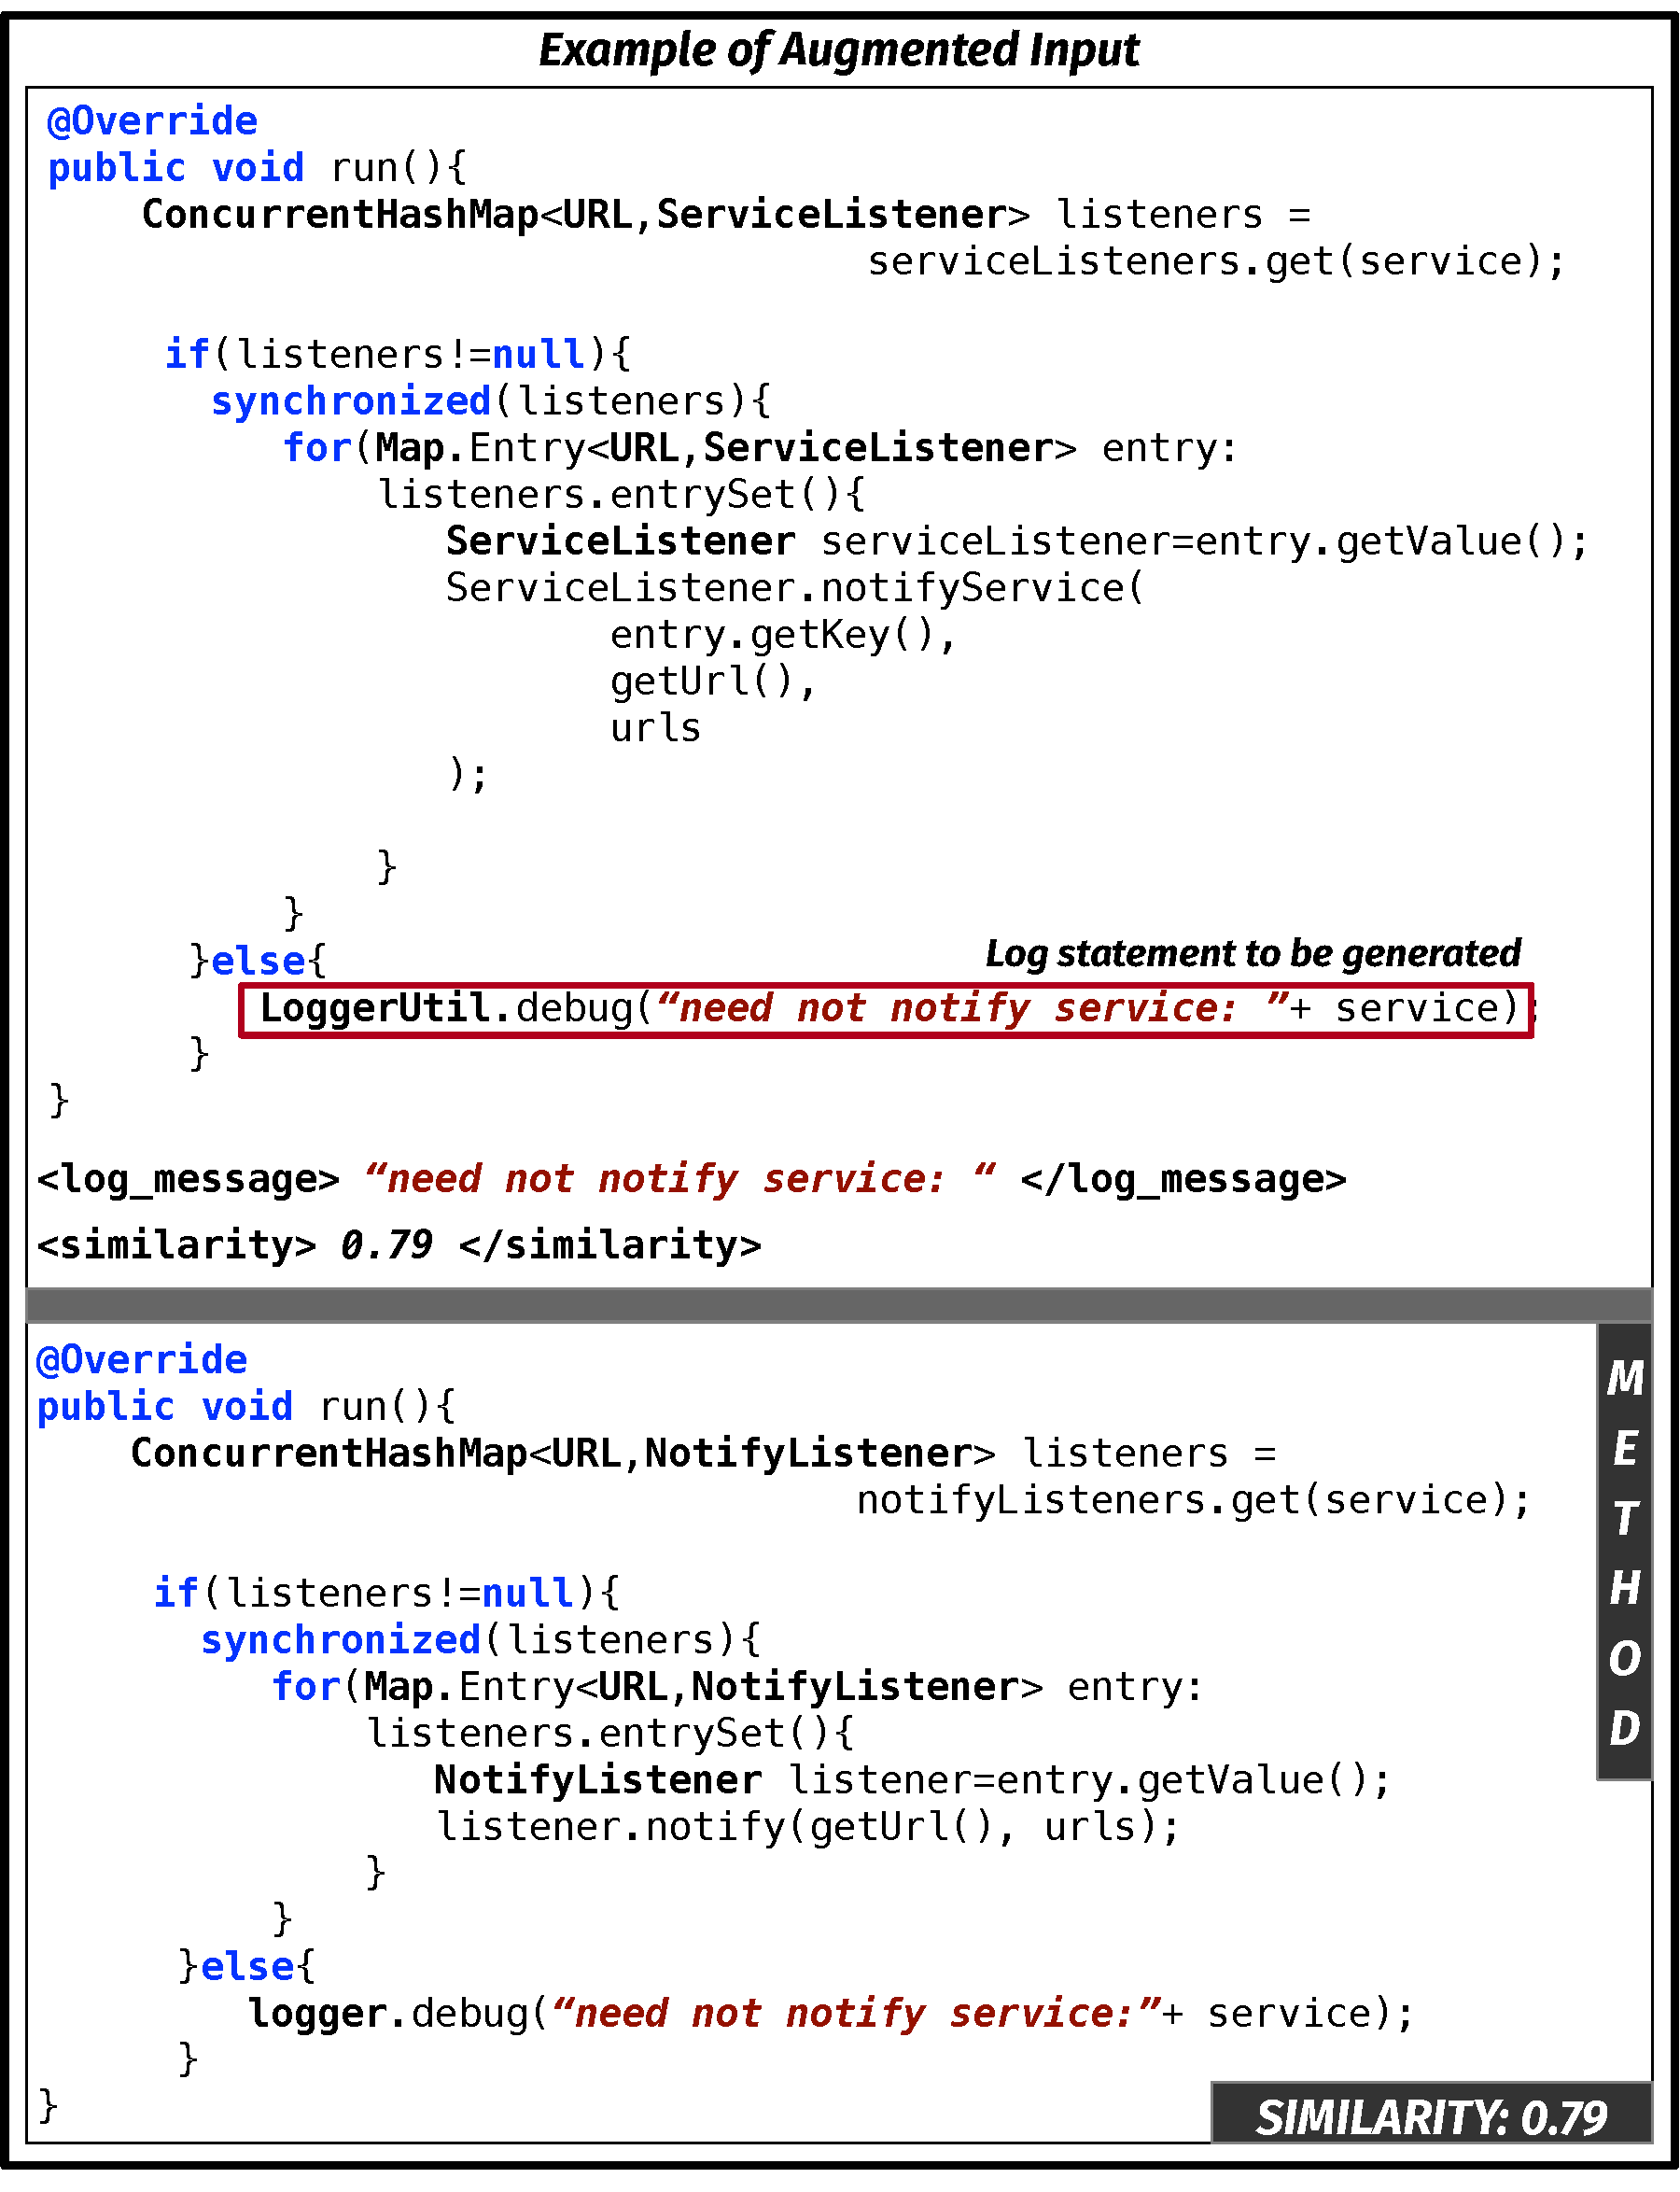
\includegraphics[width=\columnwidth]{img/ir-example.pdf}
	\caption{Example of augmented input featured by log messages retrieved from the ($k=3$) most similar coding context.}
\end{figure}

\begin{figure}[h!]
	\label{fig:pre-training}
	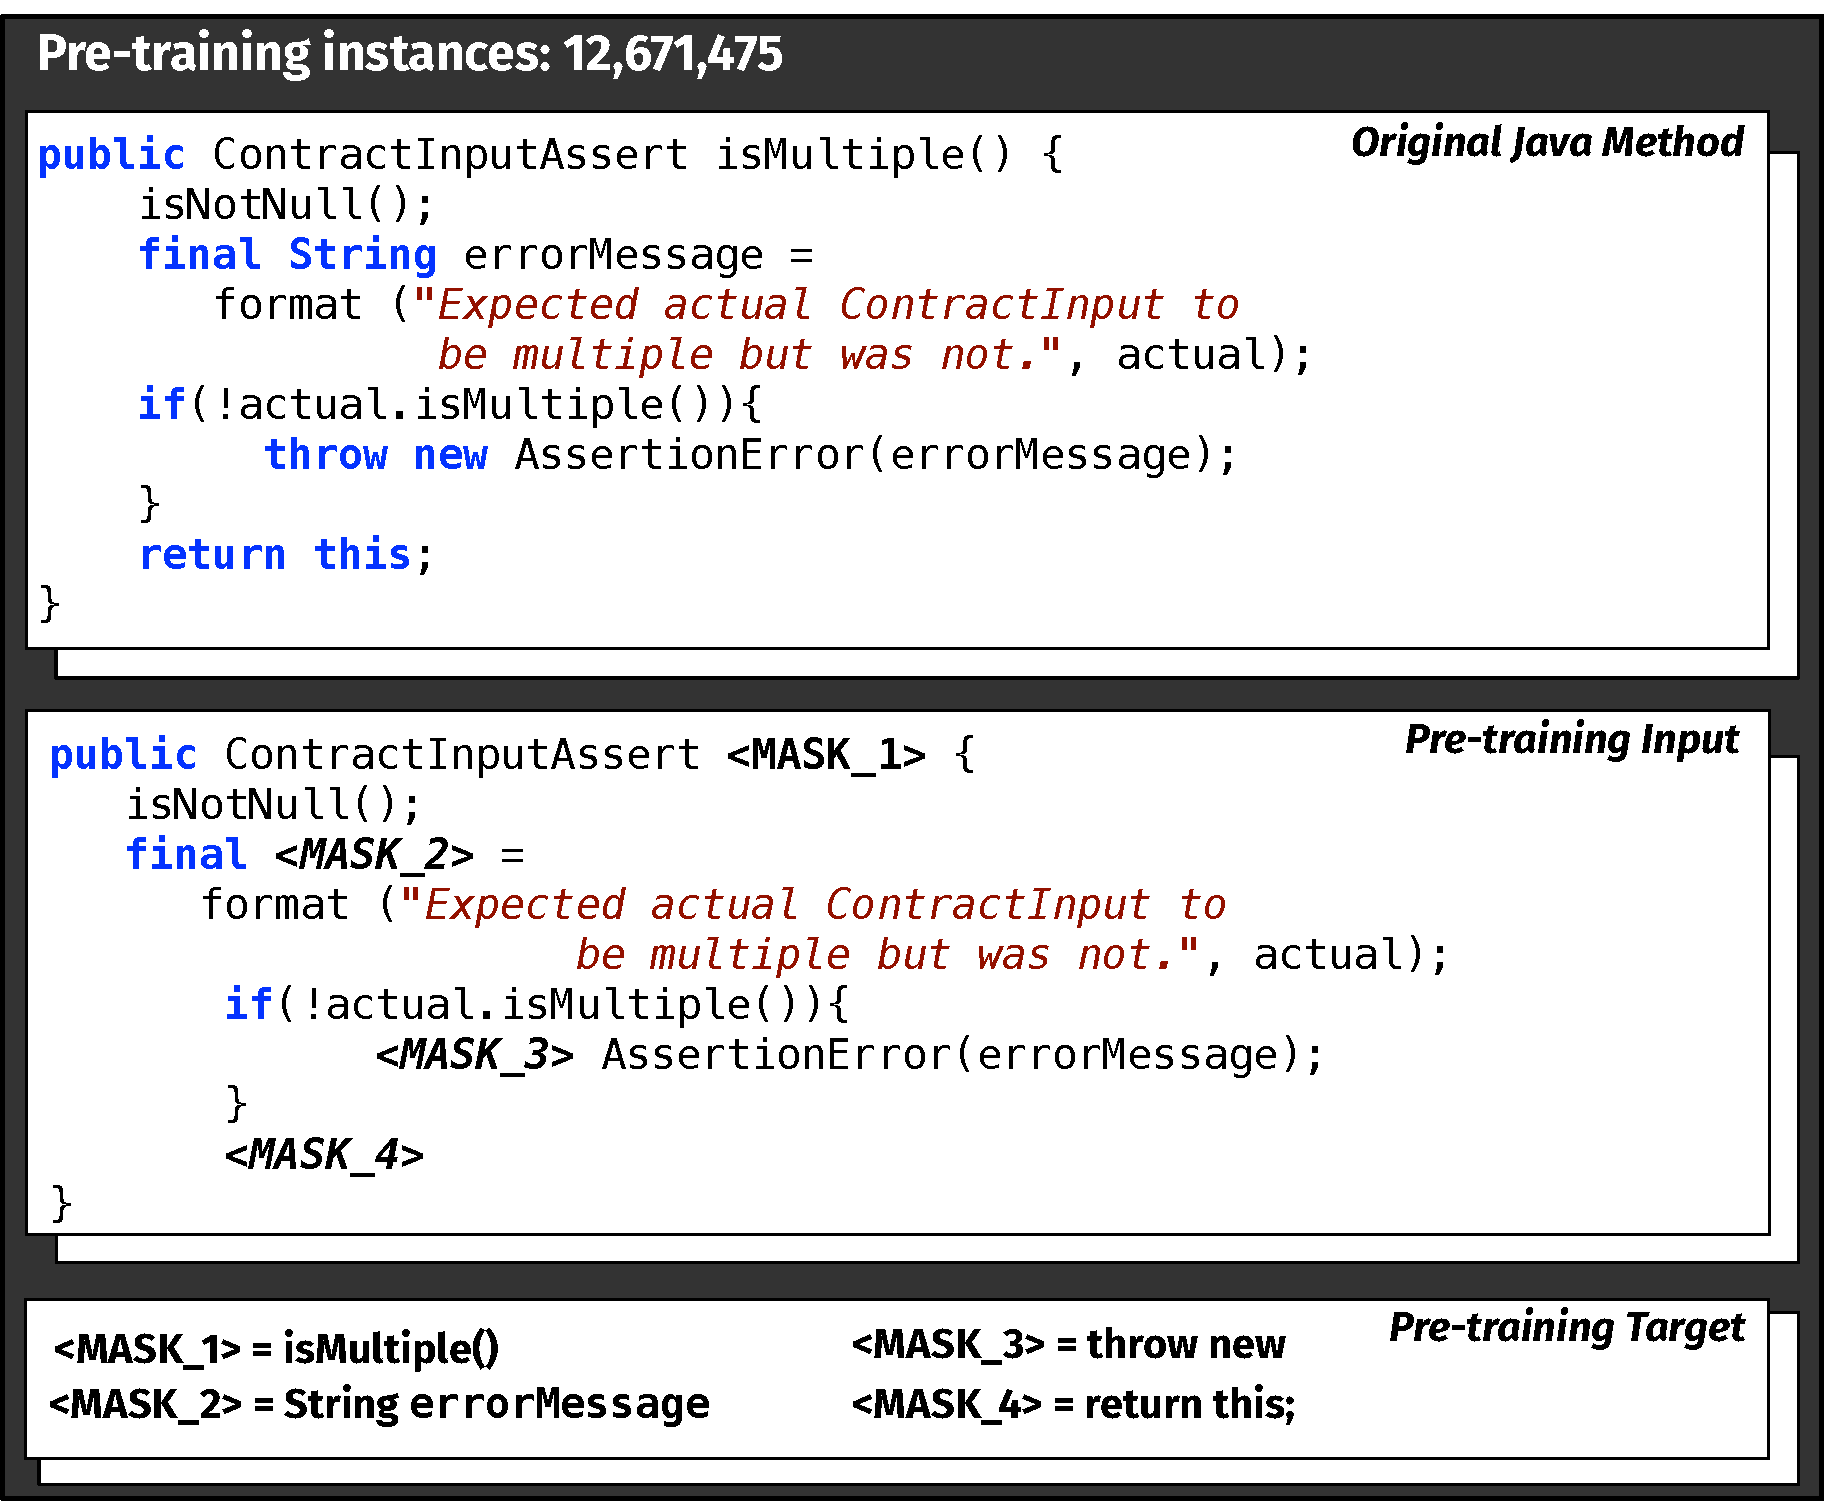
\includegraphics[width=\columnwidth]{img/pre-training.pdf}
		\caption{Example of Pre-training instance}
\end{figure}



\subsubsection{Fine-tuning Dataset: Single Log Generation} \label{sec:single-log-dataset}
We build a fine-tuning aimed at replicating what has been done in the training of LANCE by Mastropaolo \etal \cite{mastropaolo2022using}. We process each method $M$ having $n \geq 1$ log statements by removing from it one log statement (\ie leaving it with $n-1$ log statements). This allows to create a training pair $\langle M_s, M_t \rangle$ with $M_s$ representing the input provided to the model (\ie $M$ with one removed log statement) and  $M_t$ being the expected output (\ie $M$ in its original form, with all its log statements). This is the dataset used to train LANCE \cite{mastropaolo2022using} and it allows to train a model able, given a Java method as input, to inject in it one new log statement. 

For methods having $n > 1$ (\ie more than one log statement), we created $n$ pairs $\langle M_s, M_t \rangle$, each of them having one of the $n$ log statements removed (\ie different $M_s$). To ensure that after the log statement removal our instances still featured valid Java methods, we parsed each $M_s$ using JavaParser \cite{javaparser} and removed all pairs including an invalid $M_s$. 

We split the remaining pairs into training (80\%), validation (10\%) and test (10\%) set as reported in \tabref{tab:ds-summary-1}. Training and testing a T5 model on this dataset basically means performing a differentiated replication of LANCE on a much larger (+\textcolor{red}{XX\%} of instances) and more variegate (multiple logging libraries) dataset.

\subsubsection{Fine-tuning Dataset: Single Log Generation with IR} \label{sec:single-log-plus-IR}

In \approach, we want to combine DL and IR with the goal of boosting performance especially when it comes to the generation of meaningful log messages, being one of the weaknesses of LANCE. The main idea is to augment the input provided to the model (\ie $M_{s}$) with log messages belonging methods similar to $M_{s}$ which are featured in the fine-tuning training set. For each of the 244,588 $\langle M_s, M_t \rangle$ pairs in the fine-tuning dataset described in \secref{sec:single-log-dataset} (this includes training, validation, and test), we identify the $k$ most similar pairs in the training set. The similarity between two pairs is based on the similarity of their $M_s$ (\ie the method in which the log statement must be created) and it is computed using the Jaccard similarity \cite{hancock2004jaccard} index, based on the percentage of code tokens shared across the two methods. We then use these $k$ similar methods to extract from them example of log messages used in coding contexts which are similar to the $M_s$ at hand. Two clarifications are important here. First, independently if a given pair is in the training, validation, or test set, we extract its $k$ most similar pairs only from the training set. This is needed since, while predicting the log statement to inject, the training set must be the only knowledge available to the model (\ie the test set must be composed of previously unseen instances). Second, when computing the Jaccard similarity, we remove from the compared methods all log statements, since we want to identify similar ``coding contexts'' that may require similar log statements. We created three different fine-tuning datasets using different values of $k=\{1,3,5\}$ (thus, a higher/lower number of exemplar log messages provided as input to the model).




\figref{fig:ir-example} shows an example of training instance for this fine-tuning dataset. The method on top represents the $M_{s}$ \java method in which a log statement must be injected (\ie the one highlighted in red). The method is enriched with the exemplar log messages that have been found in the $k=3$ most similar methods shown in the bottom. Besides the log messages, we also provide T5 with the Jaccard similarity between the $M_{s}$ at hand (top of the figure in this case) and the method of the training set from which each log message has been extracted. This is just meant to represent an additional hint for T5 in terms of which exemplar message comes from the most similar coding context.

Note that the instances in this dataset are exactly the same of the one previously described to replicate LANCE (see \tabref{tab:ds-summary-1}). This allows a direct comparison in terms of performance which will provide information about the gain, if any, provided by the integration of the IR technique in the loop.

\subsubsection{Fine-tuning Dataset: Multi-log Injection with IR} \label{sec:multi-log-dataset}

The second limitation of LANCE \cite{mastropaolo2022using} we aim at addressing is the assumption that a Java method provided as input always require one new log statement to be injected. Also for this dataset, \approach exploits a combination of DL and IR, thus we follow a process similar to the one described in \secref{sec:single-log-plus-IR}, with the main difference being the number of log statements we ask the model to generate. In particular, given a method $M$ featuring $n$ log statements, we randomly select $y$ log statements to remove from it, with $1 \leq y \leq n$. This means that in this case we create pairs $\langle M_s, M_t \rangle$ in which $M_s$ lacks a ``random'' number of log statements that must be generated by the model to obtain the target method $M_t$. This makes the prediction task substantially more challenging as compared to the single-log injection scenario experimented in LANCE. Also in this case we parsed each $M_s$ using JavaParser \cite{javaparser} and removed all pairs including an invalid $M_s$. The remaining part of the process (\ie identifying the $k$ most similar pairs to inject examples of log messages) is exactly the same as the one described in \secref{sec:single-log-plus-IR}. \tabref{tab:ds-summary-1} shows the distribution of instances among the training, evaluation, and test set for this dataset as well.

%%%STOPPED HERE

\subsubsection{Fine-tuning Dataset: Deciding Whether Log Statements are Needed} \label{sec:predicting-dataset}

To build the dataset needed for predicting whether or not log statements are needed in a \java method, we use the same set of instances featuring the dataset built for the multi-log injection model. To this extent, we start from the original set of 244,588 \java methods having at least one log statement, then for each method, we chose an arbitrary number $k$ from 0 to $n$, where $n$ is the number of log statements in the method. Then, we randomly selected $k$ log statements out of the
method's $n$ logs. When $k$ is equal to 0 it means that no log statements have been removed and, thus, the input sequence and the target sequence are equal (\ie, the original \java method). After the log statements removal, we ensured that the input sequences still represented a valid \java code by using JavaParser \cite{javaparser} to parse the methods. All those instances throwing parsing exceptions have been removed from the datasets. 
Finally, for each instance, we replaced the target sequence with a binary choice either \texttt{Need} or \texttt{No need}. Instances labeled as \texttt{No need} correspond to the entries for which no log statements have been removed (\ie $k=0$) thus, need no further logs. On the other hand, the entries labeled as \texttt{Need} are those missing at least one log statement. It is possible that two methods differ only because they contain a different log statements, if said statements are removed then the methods could be considered equal. Thus, input sequences pointing to the same target sequences (\ie \texttt{Need}), have been removed to avoid duplicated entries in the dataset obtaining a training and a validation set feature by 190,974 instances and 23,725 respectively.

As for the test set, since it is not possible to ensure it represents the real distribution of Java methods that either need or do not need log statements, we decided to test the model's performance on three different test sets. Each test set contains a different distribution in terms of Java methods that need the injection of further logs or not. To this extent, we create three distributions:  (i) 50-50 (50\% of the instances require at least one additional log statement, the other 50\% do not), (ii) 75-25 (75\% of the methods want at least one additional log statement while the remaining 25\% do not) and, (iii) 25-75 (25\% of the instances need the injection of at least one log statements, while the other 75\% need none).
\tabref{tab:ds-summary-2} reports the number of instances contained in the above-mentioned datasets.

\begin{table*}[h!]
	\centering
	\caption{Num. of methods in the datasets used to predict the need for logs}
	\begin{tabular}{rcccccccc}
		\hline
		\multirow{2}{*}{\textit{\textbf{Dataset}}} & \multicolumn{2}{c}{\textbf{train}} & \textbf{} & \multicolumn{2}{c}{\textbf{eval}}  & \textbf{} & \multicolumn{2}{c}{\textbf{test}}  \\ \cline{2-3} \cline{5-6} \cline{8-9} 
		& \textbf{Need} & \textbf{No need}   & \textbf{} & \textbf{Need} & \textbf{No need}   & \textbf{} & \textbf{Need} & \textbf{No need}   \\ \hline
		\textit{Need4Log fine-tuning dataset (50-50)}         & 98,848        & 92,126             &           & 12,257        & 11,468             &           & 11,627        &  11,627            \\
		\textit{Need4Log fine-tuning dataset (75-25)}         & 98,848        & 92,126             &           & 12,257        & 11,468             &           & 12,159        &  4,053             \\
		\textit{Need4Log fine-tuning dataset (25-75)}         & 98,848        & 92,126             &           & 12,257        & 11,468             &           & 3,875         &  11,627            \\ \hline
	\end{tabular}
	\label{tab:ds-summary-2}
\end{table*}

\section{Training and Hyperparameter Tuning} \label{sec:training}
In this section we outline how the pre-training and the fine-tuning phase have been conducted to support the task of complete log statements generation (\ie injection of log statements) first and, the prediction of the need for log statements while working with \java methods. Afterwards, we also outline how we found the best-performing models for both tasks, exploiting two main strategies: (i) hyperparameter tuning  and (ii) early stopping.

The goal of the pre-training phase is to teach the model generalizable knowledge that is useful for the downstream task. To this extent, we want to teach the model how to handle the most recurrent patter of \java. This is achieved by leveraging a specific pre-training objective, namely, MLM (Masked-Language-Modeling). Said objective consists in teaching the model to predict missing or masked tokens in the input. We processed the methods to obtain an input sequence in which 15\% of random tokens have been masked as depicted in \figref{fig:pre-training}.
We pre-train the T5 model for 500k steps on a dataset of 12,671,475 instances using Google Colab's 2x2, 8 cores TPU topology with a batch size of 128 and a maximum sequence length of 512.
To this extent, Mastropaolo \etal \cite{mastropaolo2022using} found out that among the different pre-training strategies they experimented with, the one above described (\ie denoising-task) led to the best results. Thus, we opted for pre-training the T5 model on a bigger dataset using the same strategy to build knowledge that can be re-used while fine-tuning the model.

Once the model has been pre-trained, we can specialize it to solve a specific problem using a fine-tuning task. The objective of LANCE \cite{mastropaolo2022using} was to investigate the extent to which  T5 represented a doable approach in generating complete log statements. More specifically, its ability to generate and inject a single log statement in a \java method. Thus, given a \java method from which we removed one log statement at a time  (\secref{sec:single-log-dataset}), the model has to predict in which position to inject the log statement, what is the correct log level and has to generate a meaningful log message as well. Thus, as output, we expect the model to return the same \java method with, however, the injected complete log statement. 

Similarly, we would expect that while fine-tuning the pre-trained model on the augmented dataset (\ie  \textit{Single-Log Context-Aware fine-tuning dataset}), the contextual information (\ie log messages alongside the Jaccard similarity values) added to the input sequences can help the model in synthesizing more accurate log messages.

Concerning the hyperparameters tuning phase, as discussed by Mastropaolo \etal \cite{mastropaolo2021studying} in their seminal work introducing T5 for code-related tasks, we did not tune the T5 model hyperparameters during the pre-training phase, because such a phase is task-agnostic, and therefore it would provide limited benefits. Instead, we conduct such a phase, using the same strategy that was used when fine-tuning LANCE  \cite{mastropaolo2022using}. Thus, we experiment with four different learning rate scheduler: (i) \textit{Constant Learning Rate} (C-LR): the learning rate is fixed during the whole training (we use $LR = 0.001$, \ie the value used in the original paper \cite{raffel2019exploring}); (ii) \textit{Inverse Square Root Learning Rate} (ISR-LR): the learning rate decays as the inverse square root of the training step (the same used for pre-training by Raffel \etal); (iii) \textit{Slanted Triangular Learning Rate \cite{howard2018universal}} (ST-LR): the learning rate first linearly increases and then linearly decays to the starting learning rate;  (iv) \textit{Polynomial Decay Learning Rate} (PD-LR): the learning rate decays polynomially from an initial value to an ending value in the given decay steps.
Table \ref{tab:learning-rates} reports all the parameters used for each scheduling strategy as evaluated in \cite{mastropaolo2022using}.

\begin{table}[h]
	\centering
	\begin{tabular}{ll}
		\hline
		\textbf{Learning Rate Type} & \textbf{Parameters}               \\ \hline
		Constant                     & \textit{LR = 0.001}               \\
		Inverse Square Root         & \textit{LR\textsubscript{starting} = 0.01}  \\
		& \textit{Warmup = 10,000}          \\
		Slanted Triangular          & \textit{LR\textsubscript{starting} = 0.001} \\
		& \textit{LR\textsubscript{max} = 0.01}       \\
		& \textit{Ratio = 32}               \\
		& \textit{Cut = 0.1}                \\
		Polynomial Decay            & \textit{LR\textsubscript{starting} = 0.01}  \\
		& \textit{LR\textsubscript{end} = 0.001}      \\
		& \textit{Power = 0.5}              \\ \hline
	\end{tabular}
	\vspace{0.2cm}
	\caption{Configurations for all the learning rate strategies used in this study}
	\label{tab:learning-rates}
\end{table}


\begin{table*}[h!]
	\centering
	\caption{T5 hyperparameter tuning results while supporting the injection of single and multi log statements. The strategy leading to the best results is reported in bold.}
	\begin{tabular}{lrrrr}
		\toprule
		\textbf{Experiment}                  																		& \textbf{C-LR}              & \textbf{ST-LR}      & \textbf{ISQ-LR}        & \textbf{PD-LR} \\
		\midrule
		\textit{Single-Log Context-Aware fine-tuning dataset} ($K=1$)                         &   24.63\%                & 25.92\%    		           & \textbf{26.55\%}           &  26.36\%         \\
		\textit{Single-Log Context-Aware fine-tuning dataset} ($K=3$)                        &   26.25\%                & 26.04\%    		           & \textbf{26.68\%}          &  26.33\%         \\
		\textit{Single-Log Context-Aware fine-tuning dataset} ($K=5$)                         &  26.24\%                & 25.69\%    		           & \textbf{26.78\%}           &  26.33\%         \\
		\bottomrule
		\textit{Multi-Log fine-tuning dataset}                       										&   21.77\%                & 20.88\%    		           & \textbf{21.84}\%           &  21.57\%         \\
		\bottomrule
		\textit{Multi-Log Context-Aware fine-tuning dataset} ($K=1$)                         &   22.62\%                & 22.19\%    		           & \textbf{22.79\%}           &  22.76\%         \\
		\textit{Multi-Log Context-Aware fine-tuning dataset} ($K=3$)                        &   22.64\%                & 22.28\%    		           & \textbf{23.05\%}          &  22.59\%         \\
		\textit{Multi-Log Context-Aware fine-tuning dataset} ($K=5$)                         &   22.71\%                & 22.14\%    		           & \textbf{22.78\%}           &  22.51\%         \\
		\bottomrule
	\end{tabular}
	
	\label{tab:hp-results}
\end{table*}

Since we use software-specific corpora to pre-train and fine-tune the model we need a new vocabulary that include the \java tokens featuring our datasets. For this reason, we trained a new tokenizer (\emph{i.e.}, a SentencePiece model \cite{kudo2018sentencepiece}) on 1M Java methods and 712,634 English sentences coming from the C4 dataset \cite{raffel2019exploring}. Similarly to what has been done by Mastropaolo \etal \cite{mastropaolo2022using}, we included English sentences to deal with complex log messages and we set the size of the resulting vocabulary to 32k word-pieces.

\subsubsection{Single Log Statements Injection}

We must anticipate that we do not perform any hyperparameters tuning while replicating LANCE on our \textit{Single-Log fine-tuning dataset}, but instead, we train our T5 model supporting the complete injection of log statements on our novel dataset, using the best configuration of hyperparameters found by Mastropaolo \etal \cite{mastropaolo2022using}. In this regard, we used the Polynomial Decay Learning Rate (PD-LR), whose parameters are reported in \tabref{tab:learning-rates}. Afterward, we used the validation datasets to gauge the model accuracy every 10,000 steps and perform early stopping, choosing a delta of 0.01, and patience of 5. In doing so, we were able to select the model after 240k steps that most likely achieved the best results in terms of generalizability while avoiding overfitting.

In contrast, to find the best-performing model when fine-tuning T5 on the \textit{Single-Log Context-Aware fine-tuning dataset}, we train 12 different models (\ie four models for each experimented $K$ value) for a total of 100k steps using a sequence length of 1024 (both input and output). In addition, we doubled the number of tokens to manage the extra contextual information (\ie log messages and Jaccard similarities) added to the input sequences. At the end of such a phase, for each $K=\{1,3,5\}$, we select the model that achieves the highest number of correct predictions (\ie cases in which the predicted output sequences are equal to the oracle).

From the achieved results reported in \tabref{tab:hp-results}, it emerges a slight gain in terms of correct predictions when using the ISR-LR scheduler across the different values of $K$. Thus, we use such a scheduler to fine-tune the models on the	\textit{Single-Log Context-Aware fine-tuning dataset}. In detail, when $K=1$, we fine-tune the T5 model for 120k steps, after which we did not find improvements in going further, resulting in the activation of the early stopping strategy. When the number of methods from which we retrieve the log messages increases (\ie $K=3$ and $K=5$), the model reaches convergence after 120k steps for $K=3$, and after 190k steps for $K=5$.

\subsubsection{Multi Log Statements Injection} \label{sec:multi-injection-model}

Concerning the multi-log injection task, we perform hyperparameters tuning for both configurations (\ie augmented data and not). This resulted in the fine-tuning of 20 T5 models achieving the results reported in \tabref{tab:hp-results} (see rows from 4 to 7). In particular, from the performances, we report in \tabref{tab:hp-results} become evident a clear trend in which the ISQ-LR scheduler outperforms all the other strategies in the set of experiments we carried out. To this extent, each model has been trained using the ISQ-LR scheduler using an early stropping strategy that stops the training if no improvements in terms of correct predictions are found after 5 evaluating the model for 5 consecutive checkpoints (a new checkpoint is saved after 10k steps of fine-tuning).
The best-performing model generating log statements using the non-augmented inputs converges after \textcolor{red}{200k} steps.
On the other hand, the models that have been fine-tuned using the augmented data (\ie log messages and the Jaccard similarities of the methods), reach convergence after 270k steps for $K=1$. In contrast, when the number of methods from which we retrieve the log messages increase (\ie $K=3$ and $k=5$), both models reach convergence after 230k steps.

\subsubsection{Predicting The Need for Log Statements}
As for predicting the need for log statements, we decided to investigate the extent to which the T5 model we pre-trained for supporting the task of complete log statements generation, can further be fine-tuned on the dataset we introduced in \secref{sec:predicting-dataset} predicting whether log statements are needed or not.
Therefore to study the feasibility of a large pre-trained language model of code (\ie T5) in supporting such a task, we first found the best configurations of hyperparameters. Later, to tame overfitting we adopt the discussed early stopping strategy, evaluating the model on the validation set every 10k steps and stopping if there are no gains in terms of accuracy after 5 consecutive rounds of evaluation.
We conducted the search of the learning strategy maximizing the accuracy, fine-tuning four different models (for 100k steps), each one of which features one of the scheduler reported in \tabref{tab:learning-rates} . From the achieved results reported in \tabref{tab:need4log-hp}, the scheduler that achieves the best results is the PD-LR. Thus, we selected such a learning strategy to fine-tune the classifier model for 30k steps, after which the early stopping strategy returns the best checkpoint.

Once the best-performing T5 based classifier has been fine-tuned, it can be queued by a model able to inject log statements into \java methods (\secref{sec:multi-injection-model}).

  \begin{table}[h!]
	\centering
	\caption{T5 hyperparameters tuning results while supporting the task of predicting the need for log statements}
	\begin{tabular}{rrrrr}
		\hline
		\textbf{Experiment}        & \textbf{C-LR} & \textbf{ST-LR} & \textbf{ISQ-LR}  & \textbf{PD-LR}  \\ \hline
		\textit{Need4Log} & 96.58\%       & 96.56\%        & 96.59\%          & \textbf{96.62\%}\\ \hline
	\end{tabular}
	\label{tab:need4log-hp}
\end{table}

\subsubsection{Generating Predictions}
Once the T5 model has been pre-trained and fine-tuned to support the task of complete log statements generation and prediction of the need for logs, it can generate predictions using different decoding strategies. In this regard, we leveraged the same schema adopted by Mastropaolo \etal \cite{mastropaolo2022using}, implementing the greedy decoding strategy. Such a decoding schema generates the final predictions by selecting at each decoding step the token with the highest probability of appearing in a specific position. In doing so, a single prediction (\ie the one maximizing the likelihood of among all the produced tokens) is generated for the input sequence we give as input to the model.





% !TEX root = main.tex
%%%%%%%%%%%%%%%%%%%%%%%%%%%%%%%%%%%%%%%%
%%%%%%%%%%%%%%%%%%%%%%%%%%%%%%%%%%%%%%%%
\section{Study Design} \label{sec:design}
%%%%%%%%%%%%%%%%%%%%%%%%%%%%%%%%%%%%%%%%
%%%%%%%%%%%%%%%%%%%%%%%%%%%%%%%%%%%%%%%%

The \emph{goal} of our study is to evaluate the performance of \approach in supporting logging activities in \java methods. In particular, we focus on three scenarios: single log injection, in which we compare with the state-of-the-art approach LANCE \cite{mastropaolo2022using}; multi-log injection; and deciding wether log statements are needed or not in a given \java method. The context is represented by the test datasets reported in \tabref{tab:ds-summary-1} (for single and multi-log injection) and \tabref{tab:ds-summary-2} (for deciding whether logging is needed or not).

We aim at answering the following research questions:

\begin{itemize}

\item[\textbf{RQ$_1$:}]\textit{To what extent is \approach able to correctly inject a single complete logging statement in Java methods?} RQ$_1$ mirrors the study performed by Mastropaolo \etal~\cite{mastropaolo2022using} when presenting LANCE. In particular, we experiment \approach in the same scenario presented in \cite{mastropaolo2022using}: The injection of a single log statement in a given Java method. We compare the performance of \approach with that on LANCE when training and testing them on the same dataset. 

\item[\textbf{RQ$_2$:}]\textit{To what extent is \approach able to correctly inject multiple log statements when needed?} RQ$_2$ tests our approach in the most challenging scenario of generating and injecting from 1 to $n$ log statements in a \java method as needed.

\item[\textbf{RQ$_3$:}]\textit{To what extent is \approach able to properly decide when to inject log statements?} RQ$_3$ analyzes the accuracy of \approach in predicting whether or not log statements are needed in a given \java method, a problem that was oversaw in the work presenting LANCE \cite{mastropaolo2022using}.

\end{itemize}

\subsection{Data Collection and Analysis}

To answer RQ$_1$ we run both \approach and LANCE against the test set described in \tabref{tab:ds-summary-1} for the single log generation task. The only difference is that LANCE has been trained on the dataset not featuring the exemplar log messages added through IR (\ie the row \emph{Fine-tuning: Single Log Generation} in \tabref{tab:ds-summary-1}), while \approach exploits this information (row \emph{Fine-tuning: Single Log Generation with IR} in \tabref{tab:ds-summary-1}). However, the training and test instances are exactly the same, allowing for a direct comparison.

We assess the performance of the two techniques using the same evaluation schema of Mastropaolo \etal~\cite{mastropaolo2022using}. In particular, we contrast the predictions generated by the two models against the expected output (\ie the \java method provided as input with the addition of the correct log statement). Note that generating and injecting a log statement  (\eg \texttt{LoggerUtil.debug("execution ok")}) involves correctly predicting several information: (i) the name of the variable used for the logging (\ie \texttt{LoggerUtil}); (ii) the log level (\ie \texttt{debug}); (iii) the log message (\ie \texttt{"execution ok"}); and (iv) the position in the method in which the log statement must be injected. Thus, when a prediction is generated by the experimented models, three scenarios are possible:

\begin{description}
	\item[Correct prediction:] A prediction that correctly captures all above-described information, \ie it matches the name used for the variable, the log level, message, and position as written by the original developers.

	\item[Partially correct prediction:] A prediction that correctly captures a subset of the needed information (\eg it correctly generates the log statement but it injects it in the wrong position).

	\item[Wrong prediction:] None of the above-described information is correctly predicted.
\end{description}

As shown by Mastropaolo \etal~\cite{mastropaolo2022using}, the prediction of the log message is the most challenging part since, to correctly predict it, it requires the model to synthesize a message using the same terminology adopted by the original developers. Also, automatically assessing the correctness of the prediction for what concerns the log message is quite limitative considering that a message generated by a model using a different terminology as compared to the target log statement but being semantically equivalent to it is considered wrong. For this reason, we answer RQ$_1$ through the following combination of quantitative and qualitative analysis. On the quantitative side, we report for both \approach and LANCE the percentage of correct, partially correct, and wrong predictions. For the partially correct, we report the percentage of cases in which each of the ``log statement components'' (\ie variable name, log level, log message, and log position) has been correctly predicted. As for the percentage of correct and partially correct predictions, we pairwise compare them among the experimented techniques, using the McNemar's test \cite{mcnemar}, which is a proportion test suitable to pairwise compare dichotomous results of two different treatments. We complement the McNemar's test with the Odds Ratio (OR) effect size. We use the Holm's correction procedure \cite{Holm1979a} to account for multiple comparisons. Finally, we also compute the complementarity between LANCE and LEONID. 
To this extent, we report the percentage of perfect predictions achieved by LANCE and LEONID that are in common, that only LANCE was able to generate and to close the circle, the perfect predictions that only LEONID was capable of synthesizing.



Concerning the quality of the log messages generated by the two techniques, looking for exact matches (\ie cases in which the generated log message is identical to the one written by developers) is quite limitative considering that a prediction including a message different but semantically equivalent to the target one could still be valuable. For this reason, we also compute the following four metrics used in Natural Language Processing (NLP) for the assessment of automatically generated text:

\textbf{BLEU}~\cite{papineni2002bleu} assesses the quality of the automatically generated text by comparing it to the target text. The BLEU score ranges between 0 (the sequences are completely different) and 1 (the sequences are identical) and can be computed considering four different sizes $n$. In detail, for given a size $n$, the candidate (\ie automatically generated text) and target texts are broken into \textit{n}-grams and the algorithm determines how many \textit{n}-grams of the candidate text overlap in the target text. We report different  BLEU-\{1, 2, 3, 4\} and their geometric mean (\ie BLEU-A).

\textbf{METEOR}~\cite{meteor} is a metric based on the harmonic mean of unigram precision and recall. Compared to BLEU, METEOR uses stemming and synonyms matching to better match the human perception of sentences with similar meanings. Also in this case values range from 0 to 1, with 1 being a perfect match.

\textbf{ROUGE}~\cite{lin2004rouge} is a set of metrics focusing on automatic summarization tasks. We use the ROUGE-LCS (Longest Common Subsequence) variant which returns three values: the recall computed as \textit{LCS(X,Y)/length(X)}, the precision computed as \textit{LCS(X,Y)/length(Y)}, and the F-measure computed as the harmonic mean of recall and precision where \textit{X} and \textit{Y} represent two sequences of tokens.

\textbf{LEVENSHTEIN Distance}~\cite{levenshtein1966} provides an indication of the percentage of words that must be changed in the synthesized log message to match the target log message. This is accomplished by computing the normalized token-level Levenshtein distance \cite{levenshtein1966} (NTLev) between the predicted log message ($LM_p$) and the target log message ($LM_t$).

% Un-comment if we have space
%$$
%NTLev(LM_p, LM_t) = \frac{\mathit{TLev}(LM_p, LM_t)}{\max({\{}|LM_p|, |LM_t|\})}
%$$
%
%\noindent with $\mathit{TLev}$ representing the token-level Levenshtein distance between the two log messages. 

Such a metric can act as a proxy to estimate the effort requested to a developer in editing a non-perfect log message suggested by the model into the target one.

We also statistically compare the distribution of the BLEU-4 (computed at sentence level), METEOR, ROUGE, and LEVENSHTEIN distance related to the predictions generated by \approach and LANCE. We assume a significance level of 95\% and use the Wilcoxon signed-rank test \cite{wilcoxon}, adjusting $p$-values to account for multiple comparisons using the Holm's correction procedure \cite{Holm1979a}. The  Cliff's Delta ($d$) is used as effect size measure \cite{Gris2005a}. We follow well-established guidelines to interpret the effect size: negligible for $|d| < 0.10$, small for $0.10 \le |d| < 0.33$, medium for $0.33 \le |d| < 0.474$, and large for $|d| \ge 0.474$ \cite{Gris2005a}.

On the qualitative side, we manually inspected 300 of the partially correct predictions generated by both techniques and having all information but the log message correctly predicted. The goal of the inspection was to verify whether the generated log message, while different from the target one, was semantically equivalent to it. To this aim, two of the authors independently inspected all 600 log messages (300 for each approach), with $\sim$11\% (70) arisen conflicts being solved by a third author. We report the percentage of ``wrong'' log messages generated by both techniques classified as semantically equivalent.

To answer RQ$_2$ and evaluate the extent to which \approach is able to correctly inject multiple log statements, we run \approach against the test set reported in \tabref{tab:ds-summary-1} (see row \emph{Fine-tuning: Multi-log Injection with IR}). We then report the percentage of correct predictions generated by the approach (\ie methods for which all $n$ log statements that \approach was supposed to generate and inject have been correctly predicted). In this case we do not compute the partially correct predictions since, if a prediction is not completely correct, it is not possible to match the generated log statements with the target ones to compare them. To make this concept more clear, let us assume the case in which \approach was supposed to generate two log statements $s_1$ and $s_2$ but it only injects one statement $s_i$, being different from both $s_1$ and $s_2$. We cannot know whether $s_i$ should be compared with $s_1$ or with $s_2$ to assess the percentage of partially correct predictions in terms of \eg log level. For this reason, we only focus on the predictions being 100\% correct (\ie the method generated in output is identical to the target one). We complement this quantitative analysis with qualitative examples of predictions.

To answer RQ$_3$, we run \approach against the four test sets presented in \tabref{tab:ds-summary-2}, reporting the confusion matrix of the generated predictions and the corresponding values for accuracy, recall, and precision. We compare these results with those of two constant classifiers and a random classifier. The \emph{optimistic} constant classifier always predicts \emph{true} (\ie the method is in need of log statements), while the \emph{pessimistic} one always predicts \emph{false} (\ie the method does not need log statements). The random classifier just randomly predicts \emph{true} or \emph{false} for each input instance. \ANTONIO{ We use the same statistical analysis described for RQ$_1$ to compare \approach with the baselines. Make sure here if we have enough space to fit the table, eventually}
% !TEX root = main.tex
%%%%%%%%%%%%%%%%%%%%%%%%%%%%%%%%%%%%%%%%
%%%%%%%%%%%%%%%%%%%%%%%%%%%%%%%%%%%%%%%%
\section{Results Discussion} \label{sec:results}
%%%%%%%%%%%%%%%%%%%%%%%%%%%%%%%%%%%%%%%%
%%%%%%%%%%%%%%%%%%%%%%%%%%%%%%%%%%%%%%%%

We start by contrasting the performances of LEONID and LANCE (\secref{sec:rq1}). We follow the quantitative analysis by presenting qualitative examples of partially correct predictions in which only the log message synthesized by LEONID is wrong, while the other information (\ie variable, log level, position) are correctly predicted, but still meaningful as suggestion for developers. Then, we outline the results achieved by LEONID when injecting multiple log statements (\secref{sec:rq2}). Finally, \secref{sec:rq3} presents the results achieved by LEONID when deciding whether or not log statements are needed in a given \java method.


\subsubsection{Performance of LEONID in injection single complete log statements in \java methods (RQ$_{1}$)}
\label{sec:rq1}

\tabref{tab:single-train-results} reports the results achieved by the LEONID and LANCE, in terms of correct and partially correct predictions. We report the correct predictions for all combinations of the four ``components'' to predict (\ie log variable, log level, position where to inject it, and log message). To this extent, we analyze cases in which both LEONID and LANCE managed to correctly inject a log statement in a \java method and cases in which  at least one of the four components to predict was correct (\ie partially correct prediction).
To facilitate the reading of \tabref{tab:single-train-results}, we briefly explain how to symbols featuring it.
Each row can includes only two out of three symbols: (i) the check mark (\cmark) indicates that the results reported in that row refer to log statements in which the component ($c$) was correctly predicted. The dash mark ($-$), instead, indicates that $c$ can be either correct or wrong for the predictions in that row. Finally, the cross mark (\xmark) indicates that the component was wrongly predicted for the corresponding log statements.
For instance, the last row of \tabref{tab:single-train-results} reports the results achieved by LEONID and LANCE, when the two models correctly synthesized the log variable name, the log level and the entire the log statement has been injected in the correct position. In such a case however, the log message has been wrongly predicted, as it can be seen thanks the cross mark (\xmark) in the log message column.

The last two columns of \tabref{tab:single-train-results} report the $p$-value and the Odds Ration (OR) effect size we compute using the Mc-Nemar's test \cite{mcnemar}.

By Comparing the correct predictions (\ie first row of \tabref{tab:single-train-results}) achieved by LEONID and LANCE, it emerges that LEONID performs slightly better than LANCE, achieving 27.26\% of correct predictions, against 26.79\% achieved by LANCE.  As it can be seen, the (adjusted) $p$-value indicates a statistically significant difference, with LEONID having 1.12 higher odds to provide a correct prediction compared to LANCE. 
As for the other ``components'', what emerges is that LEONID perform slightly worse compared to LANCE.
This is true especially, for the log variable name, the log level and when considering, both components along with the log position (\ie last raw of \tabref{tab:single-train-results}). 
In these cases, the (adjusted) $p$-values indicate a statistically significant difference with ORs ranging between 0.80 to 0.91 in favor of LANCE.  Concerning the log messages and the position where the log statements have been injected, LEONID performs better than LANCE.
In detail, we found out that LEONID can generate 31.55\% of correct log messages while LANCE achieves 30.16\% of correct generated log messages. The Mc-Nemar's test computed for such component, indicates a statistically significant difference ($p$-value $<$ 0.01), with LEONID being 1.36 more likely than LANCE when generating a log messages as a real developer would do.

For the position of log statements, the difference between the two models are almost negligible. To this extent, LEONID can correctly injects log statements in \java method in 82.35\% of cases as compared to LANCE, which achieves 82.28\%. Such small differences are also captured by the statistical test we performed, for which the high $p$-value of 0.71 fails in pointing out any statistically significant difference between the two distributions.

As for the quality of the log messages, \tabref{tab:log-messages-stats} reports the results computed using the four NLP metrics presented in (\secref{sec:design}) for both models: LANCE and LEONID. For the latter, we report the results when different coding contexts (\ie $k=1$, $k=3$ and $k=5$) are used. 

In detail, we first report the BLEU score computed at corpus level, then we also report the METEOR metric and to conclude the ROUGE-LCS metric and the LEVENSHTEIN distance complement the set of NLP-related metrics we decide to use for evaluating the quality of the log messages.

By analyzing \tabref{tab:log-messages-stats}, the first thing that leap to eyes is the difference in terms of BLEU-A when comparing the performances achieved by LANCE against LEONID. In particular, as the coding context increases, such a difference tends to become more pronounced, with gains ranging between 2.8 to 3.6 percentage points in favor of LEONID. A similar trend is found when looking at different overlapping $n$-grams (\ie BLEU-1, BLEU-2, BLUE-3 and BLEU-4) as well. 

Focusing on the METEOR score, we found LEONID to generate log messages that are more likely to be perceived of higher quality by humans \cite{meteor}, as compared to LANCE, with scores that on average are 1.5\% higher. We speculate that such a result is the consequence of force-feeding the model with log messages from which can learn from and thus recommend more meaningful log messages.

As for the ROUGE-LCS, it emerges that when augmenting the input instances with log messages coming from the training set, the performances achieved by LEONID with different coding context, are always higher than LANCE, with the highest value of 44.33 points achieved with a coding context of $k=5$ as compared to 42.19 points obtained by LANCE.

Finally, the Normalized LEVENSHTEIN distance indicates how log messages produced by LEONID ($k=5$), would require up to 41.85\% of changes to match the ones written by developers. If contrasting such a result with the LEVENSHTEIN distance computed for LANCE, we realize that (on average) the number of words that a developer is asked to change is 44.02\% higher when using LANCE as compared to LEONID.

We complement the discussion of the NLP-related metrics by performing the Wilcoxon signed-rank test \cite{wilcoxon}, adjusting $p$-values to account for multiple comparisons using the Holm's correction procedure \cite{Holm1979a}. 
From the results we report in \tabref{tab:test-wilcoxon}, it comes to light how for each metric, we always have difference stastistically significant, with a negligible effect size for all the metrics, in favor of LEONID (for the Levenshtein distance a positive d is in favor of LEONID, as it is a distance). 

%if we have space put this back
%\begin{figure*}[h]
%	\centering
%	\label{fig:rq1-message-stats}
%	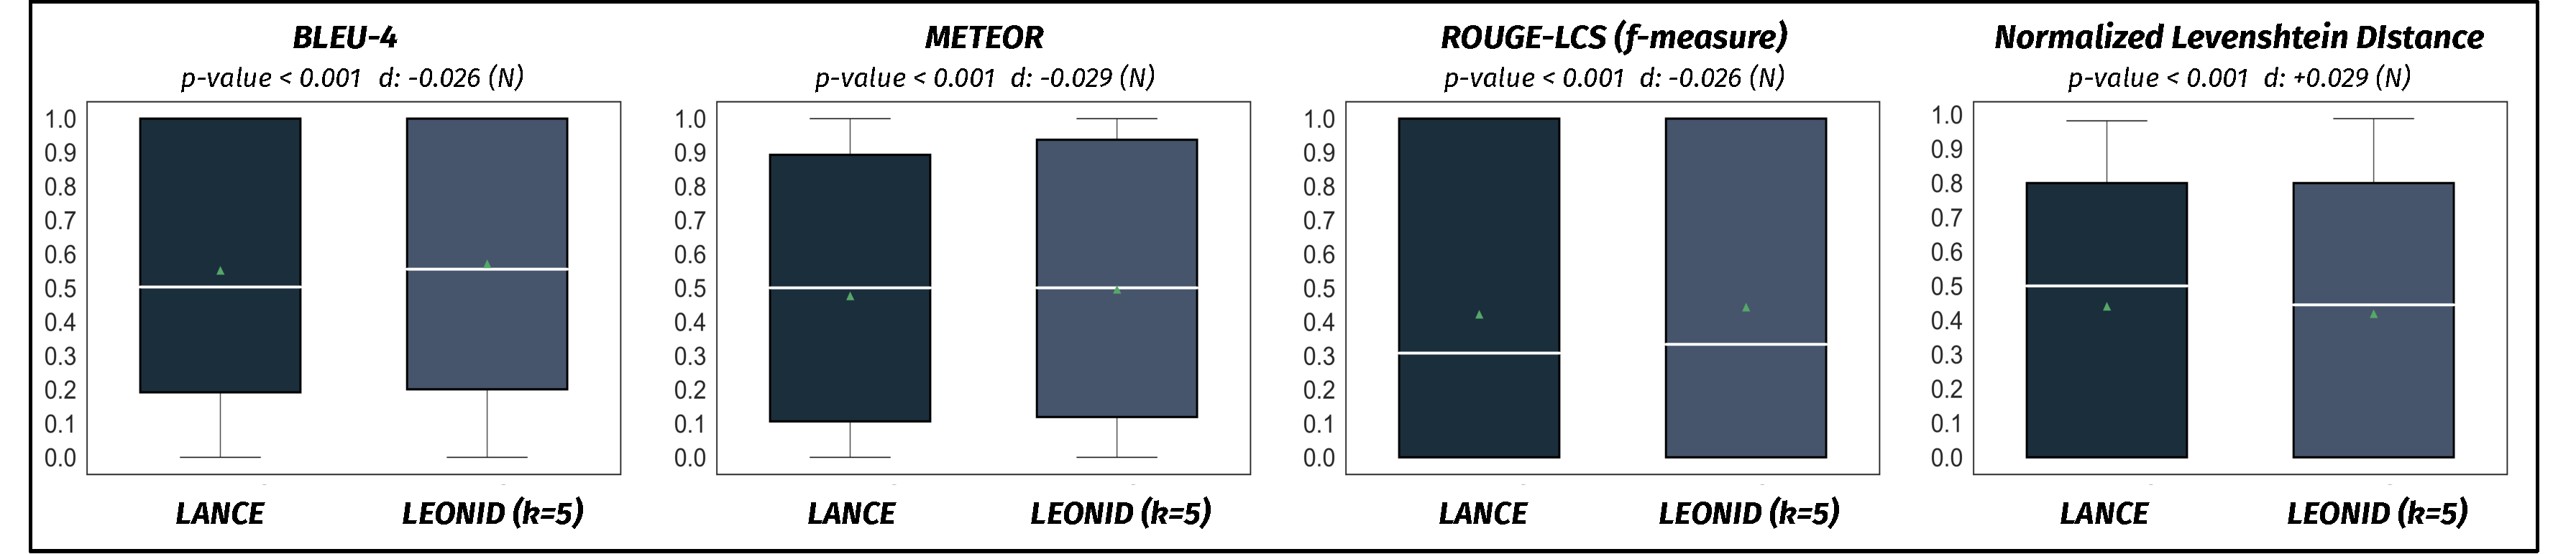
\includegraphics[width=\textwidth]{img/RQ1-log-message-boxplot.pdf}
%	\caption{Characteristics of log messages synthesized by LANCE and LEONID (K=5)}
%\end{figure*}



\begin{table}[h!]
  \centering
  \caption{Correct predictions considering the four-dimensional challenges of injecting log statements.}
  \resizebox{.5\textwidth}{!}{
	  \begin{tabular}{cccccrrrr}
	  \hline
	  Variable   & Level     & Message   & Position  &  & \multicolumn{1}{c}{LEONID} & \multicolumn{1}{c}{LANCE} & \multicolumn{1}{c}{$p$-value} & \multicolumn{1}{c}{OR}     \\ \hline
	  \ding{51}  & \ding{51} & \ding{51} & \ding{51} &  & 27.26\%                    & 26.78\%                   &                           &                            \\
	  \ding{51}  & -         & -         & -         &  & 76.45\%                    & 77.15\%                   &                           &                            \\ 
	  -          & \ding{51} & -         & -         &  & 73.53\%                    & 74.18\%                   &                           &                            \\
	  -          & -         & \ding{51} & -         &  & 31.55\%                    & 30.16\%                   &                           &                            \\ 
	  -          & -         & -         & \ding{51} &  & 82.35\%                    & 82.28\%                   &                           &                            \\ \hline
	  \ding{51}  & \ding{51} & \ding{55} & \ding{51} &  & 28.14\%                    & 29.86\%                    &                           &                            \\ \hline 
	  
	  \end{tabular}
  }
  \label{tab:single-train-results}
\end{table}





\begin{table}[h]
	\centering
	\caption{Evaluation Metrics on Log Messages: LEONID \emph{vs} LANCE\vspace{-0.2cm}}
	\scriptsize
	\label{tab:log-messages-stats}
	 \resizebox{.5\textwidth}{!}{
	\begin{tabular}{lrrrrrr}
		\toprule
		& {\bf LANCE} & {\bf LEONID ($k=1$)} &  {\bf LEONID ($k=3$)} &  {\bf LEONID ($k=5$)} \\\midrule
		BLEU-A \cite{papineni2002bleu}& 31.98 & 34.86  & 35.07 & \bf 35.36\\
			\hspace{0.2cm} BLEU-1 & 47.30 &  49.10 & 49.70  & \bf 50.00\\
			\hspace{0.2cm} BLEU-2 & 36.30 & 38.70 & 39.20 & \bf 39.60\\
			\hspace{0.2cm} BLEU-3 & 33.90 &  33.53 & 34.50 & \bf 35.00\\
			\hspace{0.2cm} BLEU-4 & 31.40 & 33.53 & 31.80 & \bf 32.40\\
		METEOR \cite{meteor} & 58.60 & 60.03  & \bf 60.43 & 60.35 \\
		ROUGE-LCS \cite{lin2004rouge} &  &  & & \\
		\hspace{0.2cm} $precision$ & 42.57 & 44.67 & 44.51  & \bf 44.68\\
		\hspace{0.2cm} $recall$ & 44.04 &  45.94 & 45.80 & \bf 46.01\\
		\hspace{0.2cm} $fmeasure$ & 42.19 & 44.26 & 44.14 & \bf 44.33\\
		LEVENSHTEIN \cite{levenshtein1966} & 44.02 & 42.27  & 41.91 & \bf 41.85 \\\bottomrule
	\end{tabular} 
	\vspace{-0.2cm}
}
\end{table}

\begin{table}[ht]
	\centering
	\caption{Statistical Tests: LEONID \emph{vs} LANCE\vspace{-0.2cm}}
	\scriptsize
	\label{tab:test-wilcoxon}
	 \resizebox{.5\textwidth}{!}{
	\begin{tabular}{llrc}
		\toprule
		\textbf{Comparison} & \textbf{Metric} & \textbf{\emph{p}-value} & \textbf{d} \\ 
		\midrule
		\multirow{3}{*}{LANCE  \emph{vs} LEONID ($k=1$)} & BLEU-4 & $<$0.001 & -0.022 (N) \\ 
			& METEOR & $<$0.001 & -0.025 (N) \\
		& ROUGE-LCS (f-measure) & $<$0.001 & -0.025 (N) \\ 
		& LEVENSHTEIN & $<$0.001 & +0.023 (N) \\\midrule
		\multirow{3}{*}{LANCE  \emph{vs} LEONID ($k=3$)} & BLEU-4 & $<$0.001 & -0.026 (N) \\ 
		& METEOR & $<$0.001 & -0.029 (N) \\
		& ROUGE-LCS (f-measure) & $<$0.001 & -0.023 (N) \\ 
		& LEVENSHTEIN & $<$0.001 & +0.027 (N) \\\midrule
			\multirow{3}{*}{LANCE  \emph{vs} LEONID ($k=5$)} & BLEU-4 & $<$0.001 & -0.026 (N) \\ 
		& METEOR & $<$0.001 & -0.029 (N) \\
		& ROUGE-LCS (f-measure) & $<$0.001 & -0.026 (N) \\ 
		& LEVENSHTEIN & $<$0.001 & +0.029 (N) \\\midrule
	\end{tabular}
}
	\vspace{-0.2cm}
\end{table}


\subsubsection{Performance of LEONID in injection multiple complete log statements in \java methods (RQ$_{2}$)}
\label{sec:rq2}
As explained in \secref{sec:design}, for RQ$_{2}$ we would not be able to compute the partially correct predictions as we performed for RQ$_{1}$. For such a reason, we limit our discussion presenting the results achieved by LEONID when injecting multiple log statements in \java Methods, while reporting qualitative examples in our online appendix \cite{}. To this extent, we found out LEONID to correctly inject multiple log statements in \java methods in 23.38\% (5,634 out of 24,088) when using a ``shallow'' coding context $k=1$. Similarly, even when increasing the window of the coding context (\ie $k=3$ and $k=5$), the achieved results do not undergo major changes, with 23.35\% for $k=3$ and 23.51\% for $k=5$.


\subsubsection{Performance of LEONID in properly deciding whether or not a \java method needs log statements  (RQ$_{3}$)}
\label{sec:rq3}

\figref{fig:rq3-cm} reports the confusion matrices with their respective values of accuracy, precision and recall (on the bottom of the figure) for each test-set in \tabref{tab:ds-summary-2}.

When half of the methods need at least one log statement, and the other half do not need any (50-50 split), LEONID reports an accuracy of 0.96, while achieving a precision of 0.98 and a recall of 0.94. In contrast the \textit{optimistic} and \textit{pessimistic} classifier would achieve 0.50 of accuracy and precision, while reporting a recall of 1.0. 
The \textit{random} classifier on the same test-set (50-50), achieves 0.50 of accuracy, precision and recall (as expected). 

When testing LEONID on the 75-25 split, there is a slightly increase in terms of precision as compared to the 50-50 split, 0.98 \emph{vs} 0.99. Consequently, the accuracy loose 0.01 points (0.95) as compared to the previous 50-50 split. Instead, the recall keeps its value fixed at 0.94.
The \textit{optimistic} classifier reports a value of 0.75 for both accuracy and precision, while achieving a recall of 1.0. As expected, the \textit{pessimistic} classifier achieves 0.25 points for both accuracy and precision and, 1.0 of recall. As for the \textit{random} classifier, we found out an accuracy and a recall of 0.5, with a precision of 0.75.

When LEONID is tested in a scenario in which the number of methods requiring log statements is outweighed by the number of methods who do not need log statements (25-75 split), precision and recall achieves both 0.94. The accuracy for such a scenario is 0.97. 
On the other hand, the \textit{optimistic} classifier would achieve a recall of 1.0, with an accuracy and precision both of 0.25 that contrast the results achieved with the \textit{pessimistic} classifier, which would report a recall of 1.0,  with accuracy and precision of 0.75. On such dataset, the \textit{random} classifier would ensure a precision of 0.25, with an accuracy and recall of 0.50.

Finally, as for the test-set resembling the original distribution of \java methods we mined (2-98 split), LEONID achieves an accuracy of 0.98, and a recall of 0.96. Instead, the precision goes down to 0.51.
As for the naive classifiers, we found out that when using the \textit{optimistic}, the achieved accuracy and precision would be both of 0.02 points, with a recall of 1.0.
In contrast, the \textit{pessimistic} performs better than LEONID (as expected), achieving 0.97 of accuracy and precision, and 1.0 of recall.
The \textit{random} classifier, on the other hand, it would ensure an accuracy 0.50, a recall of 0.53, while achieving only 0.02 of precision.





\begin{figure*}[h!]
	\centering
	\label{fig:rq3-cm}
	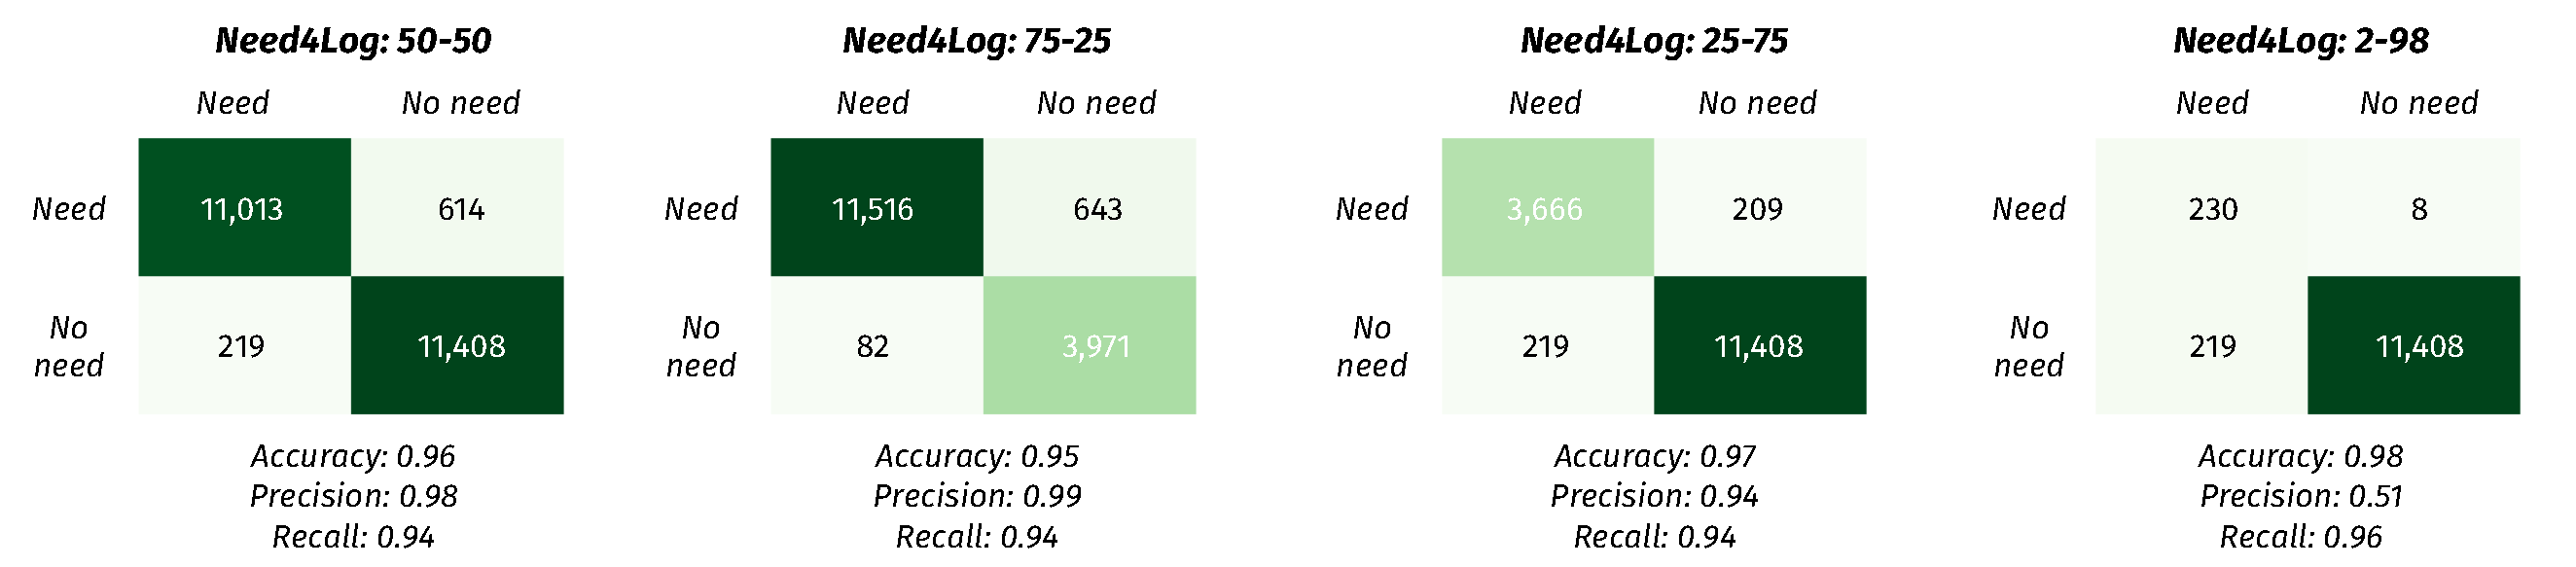
\includegraphics[width=\textwidth]{img/RQ3-CM.pdf}
	\caption{Results achieved by LEONID when deciding whether log statements are needed or not in \java methods. For each test-set (\tabref{tab:ds-summary-2}), accuracy, precision and recall are reported.}
\end{figure*}

%complementarity
%Shared:  72.05602393255371
%Only LEONID:  14.781071525700298
%Only LANCE:  13.162904541745988


% !TEX root = main.tex
%%%%%%%%%%%%%%%%%%%%%%%%%%%%%%%%%%%%%%%%
%%%%%%%%%%%%%%%%%%%%%%%%%%%%%%%%%%%%%%%%
\section{Threats to Validity} \label{sec:threats}
%%%%%%%%%%%%%%%%%%%%%%%%%%%%%%%%%%%%%%%%
%%%%%%%%%%%%%%%%%%%%%%%%%%%%%%%%%%%%%%%%

\textbf{Construct validity.} The building of our fine-tuning datasets rely on the assumption that the exploited code instances, as written by developers, represent the ``correct'' predictions that the models should generate. This is especially true for the classifier aimed at predicting whether log statements are needed. For example, the instances that we labeled as ``\emph{not needing log statements}'' are methods featuring $n \geq 1$ log statements from which we did not remove any log statement. Thus, we assume that these methods need exactly $n$ log statements (\ie the ones injected by the developers), not one more. This is a strong assumption, as confirmed by the examples in \figref{fig:no-need}. Still, using the code written by developers as oracle is a popular practice in DL for SE \cite{tufano2022using, Tufano:tosem2019, tufano-mutants, watson2020learning, tufano2022generating}.


\textbf{Internal validity.}  We performed the same hyperparameter tuning we proposed when introducing the T5 model to support code-related tasks \cite{mastropaolo2021studying}, while relying on the best architecture identified by Raffel \etal \cite{raffel2019exploring} for the other parameters. We acknowledge that additional tuning can result in improved performance.


\textbf{External validity.} Our research questions have been answered using a dataset being 3.6 times larger as compared to the dataset we originally used when proposing \cite{mastropaolo2022using}. Also, the new dataset is more variegated, featuring projects using different build systems (as compared to the Maven-only policy we relied in \cite{mastropaolo2022using}) and having dependencies towards different logging libraries (differently from the original Log4j-only policy we end up using in \cite{mastropaolo2022using}). Still, we do not claim generalizability of our findings for different populations of projects, especially those written in other programming languages.
% !TEX root = main.tex
%%%%%%%%%%%%%%%%%%%%%%%%%%%%%%%%%%%%%%%%
%%%%%%%%%%%%%%%%%%%%%%%%%%%%%%%%%%%%%%%%
\section{Related Work} \label{sec:related}
%%%%%%%%%%%%%%%%%%%%%%%%%%%%%%%%%%%%%%%%
%%%%%%%%%%%%%%%%%%%%%%%%%%%%%%%%%%%%%%%%


In recent years, DL techniques have been increasingly used to support software engineering (SE). The activities commonly supported by state-of-the-art approach include software maintenance and software testing \cite{yang2020survey}, and most of the proposed approaches target the source code \cite{watson2022systematic}. While available approaches support a plethora of concrete SE tasks \cite{yang2020survey, watson2022systematic}, in this section we focus on the ones strictly related to the target of our study: \textit{Automating Logging Activities}. A broader literature review on the topic is available in two recent surveys by Yang \etal \cite{yang2020survey} and Watson \etal \cite{watson2022systematic}.


\subsection{Empirical Studies on Logging Practices}
Yuan \etal \cite{yuan2012characterizing} conducted one of the first empirical study on logging practices in open-source systems, analyzing C and C++ projects. They show that developers make massive usage of log statements and continuously evolve them with the goal of improving debugging and maintenance activities.

Fu \etal \cite{fu2014developers} studied the logging practices in two industrial projects at Microsoft, investigating in particular which code blocks are typically logged. They also propose a tool to predict the need for a new log statement, reporting a 90\% F-Score.

Chen \cite{chen2017characterizing} and Zeng \etal \cite{zeng2019studying} extended the study of Yuan \etal \cite{yuan2012characterizing} to \java and Android systems, respectively. In particular, Chen analyzed 21 Java-based open-source projects while Zeng \etal considered 1,444 open-source Android apps mined from F-Droid. Both studies confirmed the results of Yuan \etal \cite{yuan2012characterizing}, finding a massive presence of log statements in the analyzed systems. 

Zhi \etal \cite{zhi2019exploratory} investigated how logging configurations are used and evolve, distilling 10 findings about practices adopted in logging management, storage, formatting, and configuration quality. Other researchers studied the evolution and stability  of log statements. For example, Kabinna \etal \cite{kabinna2018examining} examined how developers of four open source applications evolve log statements. They found that nearly 20-45\% of log statements change throughout the software lifetime. 

Zhou \etal \cite{zhou2020mobilogleak} explored the impact of logging practices on data leakage in mobile apps. In addition, they propose MobiLogLeak to automatically identify log statements in deployed apps that leak sensitive data. Their study show that 4\% of the analyzed apps leak sensitive data.

Recently, Li \etal~\cite{li2020qualitative} conducted an extensive investigation on logging practice from a developer's perspective. The goal of this research is to push the design of automated tools based on actual developers' needs (rather than on researchers' intuition). 

The authors surveyed 66 developers and analyzed 223 logging-related issue reports shedding light on the trade-off between costs and benefits of logging practices in open source. The results show that developers adopt an \emph{ad hoc} strategy to compensate costs and benefits while inserting logging statements for various activities (\eg debugging). 

The above-described papers lay the empirical foundations for techniques supporting developers in logging activities (including our work). Approaches such as \tool can help in reducing the cost of logging while supporting developers in taking proper decisions when they wish to add log statements.


\subsection{Automating Logging Activities}

%Zhu \etal~\cite{zhu2015learning} pioneered the research in this area presenting \textsc{LogAdvisor}, a tool to recommend where to inject log statements. The authors evaluated \textsc{LogAdvisor} on two Microsoft systems and two open-source projects, reportinga 60\% accuracy when the tool is triggered to inject log statements on pieces of code without log statements.
%
%Yao \etal~\cite{yao2018log4perf} focused on a similar sub-problem: Their approach (Log4Perf) suggests log locations for the performance monitoring of web-based systems. The evaluation showed the ability of Log4Perf to identify locations in code having a statistically significant influence on performance.
%
%Mizouchi \etal \cite{mizouchi2019padla} presented \textsc{PADLA}, an extension of Apache Log4j aimed at dynamically changing the level of log statements to optimize the amount of information logged at runtime (\eg more verbose in case of performance anomalies).
%
%Li \etal~\cite{li2020shall} were the first proposing the usage of DL to support logging. Their approach aims at recommending logging locations and can achieve 80\% accuracy in the within-project setting, and 67\% in the cross-project scenario.
%
%Li \etal \cite{li2021deeplv} lately proposed \textsc{DeepLV}, a tool to ``refactor'' the level of existing log statements in Java methods. \textsc{DeepLV} exploits both syntactic and semantic code information, and achieved new state-of-the-art results for such a task.
%
%Lastly, Mastropaolo \etal~\cite{mastropaolo2022using} introduced \textsc{LANCE}, a tool to inject complete log statements by automatically selecting a proper log level, log message and log location. We discussed the limitations of \textsc{LANCE} in \secref{sec:intro} and explained how we tried to partially overcome them. 

Researchers proposed techniques and tools to support developers in logging activities.

\textbf{Log message enhancement.} Yuan \etal \cite{yuan2012improving} proposed \textsc{LogEnhancer} as a prototype to automatically recommend relevant variable values for each log statement, refactoring its message to include such values. Their evaluation on eight systems demonstrates that \textsc{LogEnhancer} can dramatically reduce the set of potential root failure causes when inspecting log messages. Liu \etal \cite{liu2019variables} tackled the same problem using, however, a customized deep learning network. Their evaluation showed that the mean average precision of their approach is over 84\%. \smallskip 

\textbf{Log placement.} Other researchers targeted the suggestion of the best code location for log statements \cite{jia2018smartlog,li2018studying,li2020towards}. For example, Zhu \etal \cite{zhu2015learning} presented \textsc{LogAdvisor}, an approach to recommend where to add log statements. The evaluation of \textsc{LogAdvisor} on two Microsoft systems and two open-source projects reported an accuracy of 60\% when applied on pieces of code without log statements.
Yao \etal \cite{yao2018log4perf} tackled the same problem in the specific context of monitoring the CPU usage of web-based systems, showing that their approach helps developers when logging.

Li \etal \cite{li2020shall} proposed a deep learning framework to recommend logging locations at the code block level. They report a 80\% accuracy in suggesting logging locations using within-project training, with slightly worst results (67\%) in a cross-project setting. C\^andido \etal \cite{candido2021exploratory} investigated the effectiveness of log placement techniques in an industrial context. Their findings (\eg 79\% of accuracy) show that models trained on open source code can be effectively used in industry. \smallskip 

\textbf{Log level recommendation.} A third family of techniques focus on recommending the proper log level (\eg error, warning, info) for a given log statement \cite{yuan2012characterizing,oliner2012advances}. Mizouchi \etal \cite{mizouchi2019padla} proposed \textsc{PADLA} as an extension for Apache Log4j framework to automatically change the log level for better record of runtime information in case of anomalies. 
The \textsc{DeepLV} approach proposed by Li \etal \cite{li2021deeplv} uses instead a deep learning model to recommend the level of existing log statements in methods. \textsc{DeepLV} aggregates syntactic and semantic information of the source code and showed its superiority with respect to the state-of-the-art. 

Lastly, in our previous work \cite{mastropaolo2022using} we introduced \textsc{LANCE}, a tool to inject complete log statements by automatically selecting a proper log level, log message and log location. 

\subsection{Combining DL and IR to Automate Code Related Tasks}
%
Although DL showed great potential in supporting various software engineering tasks~\cite{watsonSytematicLiterature2020}, recent work showed how its performance can be further boosted by combining it with IR-based techniques. Lam \etal~\cite{LamBugLocalization2017} proposed to use IR alongside DL for bug localization. The IR technique assesses the textual similarity between bug reports and code files. The DL model is then used to learn relationships between terms in the two different vocabularies (\ie bug reports \emph{vs} source code) and compute the final similarity score. The reported results show that DL and IR well-complement each other, with their combination outperforming the individual techniques used in isolation. Similarly, Choetkiertikul \etal~\cite{choetkiertikul2018predicting} proposed to combine IR and DL for identifying software components relevant for a given open issue.

Yu \etal~\cite{yu2022automated} combined DL with IR for the task of automated assertion generation. The idea is to use IR to retrieve the most similar test method to the target one for which an assert statement must be generated. If the similarity between the retrieved method and the target one is higher than a threshold, the assert of the retrieved method is reused. Otherwise, a DL-based approach is used to generate the assert.

In this work, we combine IR and DL to improve the performance of log statement generation, especially for what concerns the definition of a meaningful log message.
% !TEX root = main.tex
%%%%%%%%%%%%%%%%%%%%%%%%%%%%%%%%%%%%%%%%
%%%%%%%%%%%%%%%%%%%%%%%%%%%%%%%%%%%%%%%%
\section{Conclusions and Future Work} \label{sec:conclusions}
%%%%%%%%%%%%%%%%%%%%%%%%%%%%%%%%%%%%%%%%
%%%%%%%%%%%%%%%%%%%%%%%%%%%%%%%%%%%%%%%%

We started by discussing the limitations of LANCE \cite{mastropaolo2022using}, the state-of-the-art approach for the generation of complete log statements. LANCE always assumes that a \emph{single} log statement \emph{must} be injected in a method provided as input. It is a strong assumption considering that a method may not need logs or may need more than one log statement. Thus, we presented \approach, an extension of LANCE able to partially address these two limitations, making a further step ahead in the automation of logging activities. Moreover, we experimented a combination of DL and IR with the goal of improving the generation of meaningful log messages achieving, however, only limited improvements over LANCE. 

We are working on implementing \approach as a tool to be deployed to developers. This is the next step needed to perform \emph{in vivo} studies, thus better understanding the main weaknesses of current DL-based log generation. 
%
\section{Acknowledgements}
	This project has received funding from the European Research Council (ERC) under the European Union's Horizon 2020 research and innovation programme (grant agreement No. 851720).


\bibliography{main}
\bibliographystyle{acm}

\end{document}


